\documentclass[twoside]{book}

% Packages required by doxygen
\usepackage{fixltx2e}
\usepackage{calc}
\usepackage{doxygen}
\usepackage[export]{adjustbox} % also loads graphicx
\usepackage{graphicx}
\usepackage[utf8]{inputenc}
\usepackage{makeidx}
\usepackage{multicol}
\usepackage{multirow}
\PassOptionsToPackage{warn}{textcomp}
\usepackage{textcomp}
\usepackage[nointegrals]{wasysym}
\usepackage[table]{xcolor}

% Font selection
\usepackage[T1]{fontenc}
\usepackage[scaled=.90]{helvet}
\usepackage{courier}
\usepackage{amssymb}
\usepackage{sectsty}
\renewcommand{\familydefault}{\sfdefault}
\allsectionsfont{%
  \fontseries{bc}\selectfont%
  \color{darkgray}%
}
\renewcommand{\DoxyLabelFont}{%
  \fontseries{bc}\selectfont%
  \color{darkgray}%
}
\newcommand{\+}{\discretionary{\mbox{\scriptsize$\hookleftarrow$}}{}{}}

% Page & text layout
\usepackage{geometry}
\geometry{%
  a4paper,%
  top=2.5cm,%
  bottom=2.5cm,%
  left=2.5cm,%
  right=2.5cm%
}
\tolerance=750
\hfuzz=15pt
\hbadness=750
\setlength{\emergencystretch}{15pt}
\setlength{\parindent}{0cm}
\setlength{\parskip}{3ex plus 2ex minus 2ex}
\makeatletter
\renewcommand{\paragraph}{%
  \@startsection{paragraph}{4}{0ex}{-1.0ex}{1.0ex}{%
    \normalfont\normalsize\bfseries\SS@parafont%
  }%
}
\renewcommand{\subparagraph}{%
  \@startsection{subparagraph}{5}{0ex}{-1.0ex}{1.0ex}{%
    \normalfont\normalsize\bfseries\SS@subparafont%
  }%
}
\makeatother

% Headers & footers
\usepackage{fancyhdr}
\pagestyle{fancyplain}
\fancyhead[LE]{\fancyplain{}{\bfseries\thepage}}
\fancyhead[CE]{\fancyplain{}{}}
\fancyhead[RE]{\fancyplain{}{\bfseries\leftmark}}
\fancyhead[LO]{\fancyplain{}{\bfseries\rightmark}}
\fancyhead[CO]{\fancyplain{}{}}
\fancyhead[RO]{\fancyplain{}{\bfseries\thepage}}
\fancyfoot[LE]{\fancyplain{}{}}
\fancyfoot[CE]{\fancyplain{}{}}
\fancyfoot[RE]{\fancyplain{}{\bfseries\scriptsize Generated by Doxygen }}
\fancyfoot[LO]{\fancyplain{}{\bfseries\scriptsize Generated by Doxygen }}
\fancyfoot[CO]{\fancyplain{}{}}
\fancyfoot[RO]{\fancyplain{}{}}
\renewcommand{\footrulewidth}{0.4pt}
\renewcommand{\chaptermark}[1]{%
  \markboth{#1}{}%
}
\renewcommand{\sectionmark}[1]{%
  \markright{\thesection\ #1}%
}

% Indices & bibliography
\usepackage{natbib}
\usepackage[titles]{tocloft}
\setcounter{tocdepth}{3}
\setcounter{secnumdepth}{5}
\makeindex

% Hyperlinks (required, but should be loaded last)
\usepackage{ifpdf}
\ifpdf
  \usepackage[pdftex,pagebackref=true]{hyperref}
\else
  \usepackage[ps2pdf,pagebackref=true]{hyperref}
\fi
\hypersetup{%
  colorlinks=true,%
  linkcolor=blue,%
  citecolor=blue,%
  unicode%
}

% Custom commands
\newcommand{\clearemptydoublepage}{%
  \newpage{\pagestyle{empty}\cleardoublepage}%
}

\usepackage{caption}
\captionsetup{labelsep=space,justification=centering,font={bf},singlelinecheck=off,skip=4pt,position=top}

%===== C O N T E N T S =====

\begin{document}

% Titlepage & ToC
\hypersetup{pageanchor=false,
             bookmarksnumbered=true,
             pdfencoding=unicode
            }
\pagenumbering{alph}
\begin{titlepage}
\vspace*{7cm}
\begin{center}%
{\Large erpecosystem \\[1ex]\large 1.\+0 }\\
\vspace*{1cm}
{\large Generated by Doxygen 1.8.14}\\
\end{center}
\end{titlepage}
\clearemptydoublepage
\pagenumbering{roman}
\tableofcontents
\clearemptydoublepage
\pagenumbering{arabic}
\hypersetup{pageanchor=true}

%--- Begin generated contents ---
\chapter{Namespace Index}
\section{Packages}
Here are the packages with brief descriptions (if available)\+:\begin{DoxyCompactList}
\item\contentsline{section}{\mbox{\hyperlink{namespacecom}{com}} }{\pageref{namespacecom}}{}
\item\contentsline{section}{\mbox{\hyperlink{namespacecom_1_1dlinkddns}{com.\+dlinkddns}} }{\pageref{namespacecom_1_1dlinkddns}}{}
\item\contentsline{section}{\mbox{\hyperlink{namespacecom_1_1dlinkddns_1_1atulsaurabh}{com.\+dlinkddns.\+atulsaurabh}} }{\pageref{namespacecom_1_1dlinkddns_1_1atulsaurabh}}{}
\item\contentsline{section}{\mbox{\hyperlink{namespacecom_1_1dlinkddns_1_1atulsaurabh_1_1erpecosystem}{com.\+dlinkddns.\+atulsaurabh.\+erpecosystem}} }{\pageref{namespacecom_1_1dlinkddns_1_1atulsaurabh_1_1erpecosystem}}{}
\item\contentsline{section}{\mbox{\hyperlink{namespacecom_1_1dlinkddns_1_1atulsaurabh_1_1erpecosystem_1_1configuration}{com.\+dlinkddns.\+atulsaurabh.\+erpecosystem.\+configuration}} }{\pageref{namespacecom_1_1dlinkddns_1_1atulsaurabh_1_1erpecosystem_1_1configuration}}{}
\item\contentsline{section}{\mbox{\hyperlink{namespacecom_1_1dlinkddns_1_1atulsaurabh_1_1erpecosystem_1_1loader}{com.\+dlinkddns.\+atulsaurabh.\+erpecosystem.\+loader}} }{\pageref{namespacecom_1_1dlinkddns_1_1atulsaurabh_1_1erpecosystem_1_1loader}}{}
\item\contentsline{section}{\mbox{\hyperlink{namespacecom_1_1dlinkddns_1_1atulsaurabh_1_1erpecosystem_1_1util}{com.\+dlinkddns.\+atulsaurabh.\+erpecosystem.\+util}} }{\pageref{namespacecom_1_1dlinkddns_1_1atulsaurabh_1_1erpecosystem_1_1util}}{}
\end{DoxyCompactList}

\chapter{Hierarchical Index}
\section{Class Hierarchy}
This inheritance list is sorted roughly, but not completely, alphabetically\+:\begin{DoxyCompactList}
\item \contentsline{section}{com.\+dlinkddns.\+atulsaurabh.\+erpecosystem.\+configuration.\+Base\+Configuration}{\pageref{classcom_1_1dlinkddns_1_1atulsaurabh_1_1erpecosystem_1_1configuration_1_1_base_configuration}}{}
\item \contentsline{section}{com.\+dlinkddns.\+atulsaurabh.\+erpecosystem.\+loader.\+Custom\+F\+X\+M\+L\+Loader}{\pageref{classcom_1_1dlinkddns_1_1atulsaurabh_1_1erpecosystem_1_1loader_1_1_custom_f_x_m_l_loader}}{}
\item \contentsline{section}{com.\+dlinkddns.\+atulsaurabh.\+erpecosystem.\+util.\+Erp\+Utility}{\pageref{interfacecom_1_1dlinkddns_1_1atulsaurabh_1_1erpecosystem_1_1util_1_1_erp_utility}}{}
\begin{DoxyCompactList}
\item \contentsline{section}{com.\+dlinkddns.\+atulsaurabh.\+erpecosystem.\+util.\+Erp\+Utility\+Impl}{\pageref{classcom_1_1dlinkddns_1_1atulsaurabh_1_1erpecosystem_1_1util_1_1_erp_utility_impl}}{}
\end{DoxyCompactList}
\item \contentsline{section}{com.\+dlinkddns.\+atulsaurabh.\+erpecosystem.\+loader.\+G\+U\+I\+Info}{\pageref{interfacecom_1_1dlinkddns_1_1atulsaurabh_1_1erpecosystem_1_1loader_1_1_g_u_i_info}}{}
\item \contentsline{section}{com.\+dlinkddns.\+atulsaurabh.\+erpecosystem.\+logger.\+Logger}{\pageref{interfacecom_1_1dlinkddns_1_1atulsaurabh_1_1erpecosystem_1_1logger_1_1_logger}}{}
\begin{DoxyCompactList}
\item \contentsline{section}{com.\+dlinkddns.\+atulsaurabh.\+erpecosystem.\+logger.\+Erp\+Ecosystem\+Logger}{\pageref{classcom_1_1dlinkddns_1_1atulsaurabh_1_1erpecosystem_1_1logger_1_1_erp_ecosystem_logger}}{}
\end{DoxyCompactList}
\item Application\begin{DoxyCompactList}
\item \contentsline{section}{com.\+dlinkddns.\+atulsaurabh.\+erpecosystem.\+Erpecosystem\+Application}{\pageref{classcom_1_1dlinkddns_1_1atulsaurabh_1_1erpecosystem_1_1_erpecosystem_application}}{}
\end{DoxyCompactList}
\item Application\+Runner\begin{DoxyCompactList}
\item \contentsline{section}{com.\+dlinkddns.\+atulsaurabh.\+erpecosystem.\+Erpecosystem\+Application}{\pageref{classcom_1_1dlinkddns_1_1atulsaurabh_1_1erpecosystem_1_1_erpecosystem_application}}{}
\end{DoxyCompactList}
\end{DoxyCompactList}

\chapter{Class Index}
\section{Class List}
Here are the classes, structs, unions and interfaces with brief descriptions\+:\begin{DoxyCompactList}
\item\contentsline{section}{\mbox{\hyperlink{classcom_1_1dlinkddns_1_1atulsaurabh_1_1erpecosystem_1_1configuration_1_1_base_configuration}{com.\+dlinkddns.\+atulsaurabh.\+erpecosystem.\+configuration.\+Base\+Configuration}} }{\pageref{classcom_1_1dlinkddns_1_1atulsaurabh_1_1erpecosystem_1_1configuration_1_1_base_configuration}}{}
\item\contentsline{section}{\mbox{\hyperlink{classcom_1_1dlinkddns_1_1atulsaurabh_1_1erpecosystem_1_1loader_1_1_custom_f_x_m_l_loader}{com.\+dlinkddns.\+atulsaurabh.\+erpecosystem.\+loader.\+Custom\+F\+X\+M\+L\+Loader}} }{\pageref{classcom_1_1dlinkddns_1_1atulsaurabh_1_1erpecosystem_1_1loader_1_1_custom_f_x_m_l_loader}}{}
\item\contentsline{section}{\mbox{\hyperlink{classcom_1_1dlinkddns_1_1atulsaurabh_1_1erpecosystem_1_1_erpecosystem_application}{com.\+dlinkddns.\+atulsaurabh.\+erpecosystem.\+Erpecosystem\+Application}} }{\pageref{classcom_1_1dlinkddns_1_1atulsaurabh_1_1erpecosystem_1_1_erpecosystem_application}}{}
\item\contentsline{section}{\mbox{\hyperlink{interfacecom_1_1dlinkddns_1_1atulsaurabh_1_1erpecosystem_1_1util_1_1_erp_utility}{com.\+dlinkddns.\+atulsaurabh.\+erpecosystem.\+util.\+Erp\+Utility}} }{\pageref{interfacecom_1_1dlinkddns_1_1atulsaurabh_1_1erpecosystem_1_1util_1_1_erp_utility}}{}
\item\contentsline{section}{\mbox{\hyperlink{classcom_1_1dlinkddns_1_1atulsaurabh_1_1erpecosystem_1_1util_1_1_erp_utility_impl}{com.\+dlinkddns.\+atulsaurabh.\+erpecosystem.\+util.\+Erp\+Utility\+Impl}} }{\pageref{classcom_1_1dlinkddns_1_1atulsaurabh_1_1erpecosystem_1_1util_1_1_erp_utility_impl}}{}
\item\contentsline{section}{\mbox{\hyperlink{interfacecom_1_1dlinkddns_1_1atulsaurabh_1_1erpecosystem_1_1loader_1_1_g_u_i_info}{com.\+dlinkddns.\+atulsaurabh.\+erpecosystem.\+loader.\+G\+U\+I\+Info}} }{\pageref{interfacecom_1_1dlinkddns_1_1atulsaurabh_1_1erpecosystem_1_1loader_1_1_g_u_i_info}}{}
\end{DoxyCompactList}

\chapter{File Index}
\section{File List}
Here is a list of all files with brief descriptions\+:\begin{DoxyCompactList}
\item\contentsline{section}{com/dlinkddns/atulsaurabh/erpecosystem/\mbox{\hyperlink{_erpecosystem_application_8java}{Erpecosystem\+Application.\+java}} }{\pageref{_erpecosystem_application_8java}}{}
\item\contentsline{section}{com/dlinkddns/atulsaurabh/erpecosystem/configuration/\mbox{\hyperlink{_base_configuration_8java}{Base\+Configuration.\+java}} }{\pageref{_base_configuration_8java}}{}
\item\contentsline{section}{com/dlinkddns/atulsaurabh/erpecosystem/loader/\mbox{\hyperlink{_custom_f_x_m_l_loader_8java}{Custom\+F\+X\+M\+L\+Loader.\+java}} }{\pageref{_custom_f_x_m_l_loader_8java}}{}
\item\contentsline{section}{com/dlinkddns/atulsaurabh/erpecosystem/loader/\mbox{\hyperlink{_g_u_i_info_8java}{G\+U\+I\+Info.\+java}} }{\pageref{_g_u_i_info_8java}}{}
\item\contentsline{section}{com/dlinkddns/atulsaurabh/erpecosystem/util/\mbox{\hyperlink{_erp_utility_8java}{Erp\+Utility.\+java}} }{\pageref{_erp_utility_8java}}{}
\item\contentsline{section}{com/dlinkddns/atulsaurabh/erpecosystem/util/\mbox{\hyperlink{_erp_utility_impl_8java}{Erp\+Utility\+Impl.\+java}} }{\pageref{_erp_utility_impl_8java}}{}
\end{DoxyCompactList}

\chapter{Namespace Documentation}
\hypertarget{namespacecom}{}\section{Package com}
\label{namespacecom}\index{com@{com}}
\subsection*{Packages}
\begin{DoxyCompactItemize}
\item 
package \mbox{\hyperlink{namespacecom_1_1dlinkddns}{dlinkddns}}
\end{DoxyCompactItemize}

\hypertarget{namespacecom_1_1dlinkddns}{}\section{Package com.\+dlinkddns}
\label{namespacecom_1_1dlinkddns}\index{com.\+dlinkddns@{com.\+dlinkddns}}
\subsection*{Packages}
\begin{DoxyCompactItemize}
\item 
package \mbox{\hyperlink{namespacecom_1_1dlinkddns_1_1atulsaurabh}{atulsaurabh}}
\end{DoxyCompactItemize}

\hypertarget{namespacecom_1_1dlinkddns_1_1atulsaurabh}{}\section{Package com.\+dlinkddns.\+atulsaurabh}
\label{namespacecom_1_1dlinkddns_1_1atulsaurabh}\index{com.\+dlinkddns.\+atulsaurabh@{com.\+dlinkddns.\+atulsaurabh}}
\subsection*{Packages}
\begin{DoxyCompactItemize}
\item 
package \mbox{\hyperlink{namespacecom_1_1dlinkddns_1_1atulsaurabh_1_1erpecosystem}{erpecosystem}}
\end{DoxyCompactItemize}

\hypertarget{namespacecom_1_1dlinkddns_1_1atulsaurabh_1_1erpecosystem}{}\section{Package com.\+dlinkddns.\+atulsaurabh.\+erpecosystem}
\label{namespacecom_1_1dlinkddns_1_1atulsaurabh_1_1erpecosystem}\index{com.\+dlinkddns.\+atulsaurabh.\+erpecosystem@{com.\+dlinkddns.\+atulsaurabh.\+erpecosystem}}
\subsection*{Packages}
\begin{DoxyCompactItemize}
\item 
package \mbox{\hyperlink{namespacecom_1_1dlinkddns_1_1atulsaurabh_1_1erpecosystem_1_1configuration}{configuration}}
\item 
package \mbox{\hyperlink{namespacecom_1_1dlinkddns_1_1atulsaurabh_1_1erpecosystem_1_1loader}{loader}}
\item 
package \mbox{\hyperlink{namespacecom_1_1dlinkddns_1_1atulsaurabh_1_1erpecosystem_1_1logger}{logger}}
\item 
package \mbox{\hyperlink{namespacecom_1_1dlinkddns_1_1atulsaurabh_1_1erpecosystem_1_1util}{util}}
\end{DoxyCompactItemize}
\subsection*{Classes}
\begin{DoxyCompactItemize}
\item 
class \mbox{\hyperlink{classcom_1_1dlinkddns_1_1atulsaurabh_1_1erpecosystem_1_1_erpecosystem_application}{Erpecosystem\+Application}}
\end{DoxyCompactItemize}

\hypertarget{namespacecom_1_1dlinkddns_1_1atulsaurabh_1_1erpecosystem_1_1configuration}{}\section{Package com.\+dlinkddns.\+atulsaurabh.\+erpecosystem.\+configuration}
\label{namespacecom_1_1dlinkddns_1_1atulsaurabh_1_1erpecosystem_1_1configuration}\index{com.\+dlinkddns.\+atulsaurabh.\+erpecosystem.\+configuration@{com.\+dlinkddns.\+atulsaurabh.\+erpecosystem.\+configuration}}
\subsection*{Classes}
\begin{DoxyCompactItemize}
\item 
class \mbox{\hyperlink{classcom_1_1dlinkddns_1_1atulsaurabh_1_1erpecosystem_1_1configuration_1_1_base_configuration}{Base\+Configuration}}
\end{DoxyCompactItemize}

\hypertarget{namespacecom_1_1dlinkddns_1_1atulsaurabh_1_1erpecosystem_1_1loader}{}\section{Package com.\+dlinkddns.\+atulsaurabh.\+erpecosystem.\+loader}
\label{namespacecom_1_1dlinkddns_1_1atulsaurabh_1_1erpecosystem_1_1loader}\index{com.\+dlinkddns.\+atulsaurabh.\+erpecosystem.\+loader@{com.\+dlinkddns.\+atulsaurabh.\+erpecosystem.\+loader}}
\subsection*{Classes}
\begin{DoxyCompactItemize}
\item 
class \mbox{\hyperlink{classcom_1_1dlinkddns_1_1atulsaurabh_1_1erpecosystem_1_1loader_1_1_custom_f_x_m_l_loader}{Custom\+F\+X\+M\+L\+Loader}}
\item 
interface \mbox{\hyperlink{interfacecom_1_1dlinkddns_1_1atulsaurabh_1_1erpecosystem_1_1loader_1_1_g_u_i_info}{G\+U\+I\+Info}}
\end{DoxyCompactItemize}

\hypertarget{namespacecom_1_1dlinkddns_1_1atulsaurabh_1_1erpecosystem_1_1logger}{}\section{Package com.\+dlinkddns.\+atulsaurabh.\+erpecosystem.\+logger}
\label{namespacecom_1_1dlinkddns_1_1atulsaurabh_1_1erpecosystem_1_1logger}\index{com.\+dlinkddns.\+atulsaurabh.\+erpecosystem.\+logger@{com.\+dlinkddns.\+atulsaurabh.\+erpecosystem.\+logger}}
\subsection*{Classes}
\begin{DoxyCompactItemize}
\item 
class \mbox{\hyperlink{classcom_1_1dlinkddns_1_1atulsaurabh_1_1erpecosystem_1_1logger_1_1_erp_ecosystem_logger}{Erp\+Ecosystem\+Logger}}
\item 
interface \mbox{\hyperlink{interfacecom_1_1dlinkddns_1_1atulsaurabh_1_1erpecosystem_1_1logger_1_1_logger}{Logger}}
\end{DoxyCompactItemize}

\hypertarget{namespacecom_1_1dlinkddns_1_1atulsaurabh_1_1erpecosystem_1_1util}{}\section{Package com.\+dlinkddns.\+atulsaurabh.\+erpecosystem.\+util}
\label{namespacecom_1_1dlinkddns_1_1atulsaurabh_1_1erpecosystem_1_1util}\index{com.\+dlinkddns.\+atulsaurabh.\+erpecosystem.\+util@{com.\+dlinkddns.\+atulsaurabh.\+erpecosystem.\+util}}
\subsection*{Classes}
\begin{DoxyCompactItemize}
\item 
interface \mbox{\hyperlink{interfacecom_1_1dlinkddns_1_1atulsaurabh_1_1erpecosystem_1_1util_1_1_erp_utility}{Erp\+Utility}}
\item 
class \mbox{\hyperlink{classcom_1_1dlinkddns_1_1atulsaurabh_1_1erpecosystem_1_1util_1_1_erp_utility_impl}{Erp\+Utility\+Impl}}
\end{DoxyCompactItemize}

\chapter{Class Documentation}
\hypertarget{classcom_1_1dlinkddns_1_1atulsaurabh_1_1erpecosystem_1_1configuration_1_1_base_configuration}{}\section{com.\+dlinkddns.\+atulsaurabh.\+erpecosystem.\+configuration.\+Base\+Configuration Class Reference}
\label{classcom_1_1dlinkddns_1_1atulsaurabh_1_1erpecosystem_1_1configuration_1_1_base_configuration}\index{com.\+dlinkddns.\+atulsaurabh.\+erpecosystem.\+configuration.\+Base\+Configuration@{com.\+dlinkddns.\+atulsaurabh.\+erpecosystem.\+configuration.\+Base\+Configuration}}
\subsection*{Public Member Functions}
\begin{DoxyCompactItemize}
\item 
\mbox{\hyperlink{interfacecom_1_1dlinkddns_1_1atulsaurabh_1_1erpecosystem_1_1logger_1_1_logger}{Logger}} \mbox{\hyperlink{classcom_1_1dlinkddns_1_1atulsaurabh_1_1erpecosystem_1_1configuration_1_1_base_configuration_a1e3b30da635356fabf646a14241b116d}{logger}} ()
\item 
\mbox{\hyperlink{interfacecom_1_1dlinkddns_1_1atulsaurabh_1_1erpecosystem_1_1logger_1_1_logger}{Logger}} \mbox{\hyperlink{classcom_1_1dlinkddns_1_1atulsaurabh_1_1erpecosystem_1_1configuration_1_1_base_configuration_ab280a65420b19fb7b76218a39ab6db67}{rolling\+Logger}} ()
\item 
\mbox{\hyperlink{interfacecom_1_1dlinkddns_1_1atulsaurabh_1_1erpecosystem_1_1util_1_1_erp_utility}{Erp\+Utility}} \mbox{\hyperlink{classcom_1_1dlinkddns_1_1atulsaurabh_1_1erpecosystem_1_1configuration_1_1_base_configuration_ac854d5f3ef3af3b9d6d219808815d396}{erp\+Utility}} ()
\item 
\mbox{\hyperlink{classcom_1_1dlinkddns_1_1atulsaurabh_1_1erpecosystem_1_1loader_1_1_custom_f_x_m_l_loader}{Custom\+F\+X\+M\+L\+Loader}} \mbox{\hyperlink{classcom_1_1dlinkddns_1_1atulsaurabh_1_1erpecosystem_1_1configuration_1_1_base_configuration_ad02c1d56c9b4481c9011b4c3825dd10a}{custom\+F\+X\+M\+L\+Loader}} ()
\end{DoxyCompactItemize}


\subsection{Detailed Description}
\begin{DoxyAuthor}{Author}
Atul Saurabh 
\end{DoxyAuthor}
\begin{DoxyVersion}{Version}
1.\+0 
\end{DoxyVersion}


Definition at line 25 of file Base\+Configuration.\+java.



\subsection{Member Function Documentation}
\mbox{\Hypertarget{classcom_1_1dlinkddns_1_1atulsaurabh_1_1erpecosystem_1_1configuration_1_1_base_configuration_ad02c1d56c9b4481c9011b4c3825dd10a}\label{classcom_1_1dlinkddns_1_1atulsaurabh_1_1erpecosystem_1_1configuration_1_1_base_configuration_ad02c1d56c9b4481c9011b4c3825dd10a}} 
\index{com\+::dlinkddns\+::atulsaurabh\+::erpecosystem\+::configuration\+::\+Base\+Configuration@{com\+::dlinkddns\+::atulsaurabh\+::erpecosystem\+::configuration\+::\+Base\+Configuration}!custom\+F\+X\+M\+L\+Loader@{custom\+F\+X\+M\+L\+Loader}}
\index{custom\+F\+X\+M\+L\+Loader@{custom\+F\+X\+M\+L\+Loader}!com\+::dlinkddns\+::atulsaurabh\+::erpecosystem\+::configuration\+::\+Base\+Configuration@{com\+::dlinkddns\+::atulsaurabh\+::erpecosystem\+::configuration\+::\+Base\+Configuration}}
\subsubsection{\texorpdfstring{custom\+F\+X\+M\+L\+Loader()}{customFXMLLoader()}}
{\footnotesize\ttfamily \mbox{\hyperlink{classcom_1_1dlinkddns_1_1atulsaurabh_1_1erpecosystem_1_1loader_1_1_custom_f_x_m_l_loader}{Custom\+F\+X\+M\+L\+Loader}} com.\+dlinkddns.\+atulsaurabh.\+erpecosystem.\+configuration.\+Base\+Configuration.\+custom\+F\+X\+M\+L\+Loader (\begin{DoxyParamCaption}{ }\end{DoxyParamCaption})}



Definition at line 52 of file Base\+Configuration.\+java.

\mbox{\Hypertarget{classcom_1_1dlinkddns_1_1atulsaurabh_1_1erpecosystem_1_1configuration_1_1_base_configuration_ac854d5f3ef3af3b9d6d219808815d396}\label{classcom_1_1dlinkddns_1_1atulsaurabh_1_1erpecosystem_1_1configuration_1_1_base_configuration_ac854d5f3ef3af3b9d6d219808815d396}} 
\index{com\+::dlinkddns\+::atulsaurabh\+::erpecosystem\+::configuration\+::\+Base\+Configuration@{com\+::dlinkddns\+::atulsaurabh\+::erpecosystem\+::configuration\+::\+Base\+Configuration}!erp\+Utility@{erp\+Utility}}
\index{erp\+Utility@{erp\+Utility}!com\+::dlinkddns\+::atulsaurabh\+::erpecosystem\+::configuration\+::\+Base\+Configuration@{com\+::dlinkddns\+::atulsaurabh\+::erpecosystem\+::configuration\+::\+Base\+Configuration}}
\subsubsection{\texorpdfstring{erp\+Utility()}{erpUtility()}}
{\footnotesize\ttfamily \mbox{\hyperlink{interfacecom_1_1dlinkddns_1_1atulsaurabh_1_1erpecosystem_1_1util_1_1_erp_utility}{Erp\+Utility}} com.\+dlinkddns.\+atulsaurabh.\+erpecosystem.\+configuration.\+Base\+Configuration.\+erp\+Utility (\begin{DoxyParamCaption}{ }\end{DoxyParamCaption})}



Definition at line 46 of file Base\+Configuration.\+java.

\mbox{\Hypertarget{classcom_1_1dlinkddns_1_1atulsaurabh_1_1erpecosystem_1_1configuration_1_1_base_configuration_a1e3b30da635356fabf646a14241b116d}\label{classcom_1_1dlinkddns_1_1atulsaurabh_1_1erpecosystem_1_1configuration_1_1_base_configuration_a1e3b30da635356fabf646a14241b116d}} 
\index{com\+::dlinkddns\+::atulsaurabh\+::erpecosystem\+::configuration\+::\+Base\+Configuration@{com\+::dlinkddns\+::atulsaurabh\+::erpecosystem\+::configuration\+::\+Base\+Configuration}!logger@{logger}}
\index{logger@{logger}!com\+::dlinkddns\+::atulsaurabh\+::erpecosystem\+::configuration\+::\+Base\+Configuration@{com\+::dlinkddns\+::atulsaurabh\+::erpecosystem\+::configuration\+::\+Base\+Configuration}}
\subsubsection{\texorpdfstring{logger()}{logger()}}
{\footnotesize\ttfamily \mbox{\hyperlink{interfacecom_1_1dlinkddns_1_1atulsaurabh_1_1erpecosystem_1_1logger_1_1_logger}{Logger}} com.\+dlinkddns.\+atulsaurabh.\+erpecosystem.\+configuration.\+Base\+Configuration.\+logger (\begin{DoxyParamCaption}{ }\end{DoxyParamCaption})}



Definition at line 29 of file Base\+Configuration.\+java.

\mbox{\Hypertarget{classcom_1_1dlinkddns_1_1atulsaurabh_1_1erpecosystem_1_1configuration_1_1_base_configuration_ab280a65420b19fb7b76218a39ab6db67}\label{classcom_1_1dlinkddns_1_1atulsaurabh_1_1erpecosystem_1_1configuration_1_1_base_configuration_ab280a65420b19fb7b76218a39ab6db67}} 
\index{com\+::dlinkddns\+::atulsaurabh\+::erpecosystem\+::configuration\+::\+Base\+Configuration@{com\+::dlinkddns\+::atulsaurabh\+::erpecosystem\+::configuration\+::\+Base\+Configuration}!rolling\+Logger@{rolling\+Logger}}
\index{rolling\+Logger@{rolling\+Logger}!com\+::dlinkddns\+::atulsaurabh\+::erpecosystem\+::configuration\+::\+Base\+Configuration@{com\+::dlinkddns\+::atulsaurabh\+::erpecosystem\+::configuration\+::\+Base\+Configuration}}
\subsubsection{\texorpdfstring{rolling\+Logger()}{rollingLogger()}}
{\footnotesize\ttfamily \mbox{\hyperlink{interfacecom_1_1dlinkddns_1_1atulsaurabh_1_1erpecosystem_1_1logger_1_1_logger}{Logger}} com.\+dlinkddns.\+atulsaurabh.\+erpecosystem.\+configuration.\+Base\+Configuration.\+rolling\+Logger (\begin{DoxyParamCaption}{ }\end{DoxyParamCaption})}



Definition at line 37 of file Base\+Configuration.\+java.



The documentation for this class was generated from the following file\+:\begin{DoxyCompactItemize}
\item 
C\+:/myworkplace/projects/erpecosystem/src/main/java/com/dlinkddns/atulsaurabh/erpecosystem/configuration/\mbox{\hyperlink{_base_configuration_8java}{Base\+Configuration.\+java}}\end{DoxyCompactItemize}

\hypertarget{classcom_1_1dlinkddns_1_1atulsaurabh_1_1erpecosystem_1_1loader_1_1_custom_f_x_m_l_loader}{}\section{com.\+dlinkddns.\+atulsaurabh.\+erpecosystem.\+loader.\+Custom\+F\+X\+M\+L\+Loader Class Reference}
\label{classcom_1_1dlinkddns_1_1atulsaurabh_1_1erpecosystem_1_1loader_1_1_custom_f_x_m_l_loader}\index{com.\+dlinkddns.\+atulsaurabh.\+erpecosystem.\+loader.\+Custom\+F\+X\+M\+L\+Loader@{com.\+dlinkddns.\+atulsaurabh.\+erpecosystem.\+loader.\+Custom\+F\+X\+M\+L\+Loader}}
\subsection*{Public Member Functions}
\begin{DoxyCompactItemize}
\item 
final Parent \mbox{\hyperlink{classcom_1_1dlinkddns_1_1atulsaurabh_1_1erpecosystem_1_1loader_1_1_custom_f_x_m_l_loader_a7e3c0b074c43866c2950964b208b2bef}{load}} (String gui\+Name)
\item 
final Stage \mbox{\hyperlink{classcom_1_1dlinkddns_1_1atulsaurabh_1_1erpecosystem_1_1loader_1_1_custom_f_x_m_l_loader_abd9fb19f6b3d55a6044e83db37b23fd4}{create\+Stage}} (String U\+I\+Name, String key)
\end{DoxyCompactItemize}


\subsection{Detailed Description}
\begin{DoxyAuthor}{Author}
Atul Saurabh 
\end{DoxyAuthor}
\begin{DoxyVersion}{Version}
1.\+0 
\end{DoxyVersion}


Definition at line 23 of file Custom\+F\+X\+M\+L\+Loader.\+java.



\subsection{Member Function Documentation}
\mbox{\Hypertarget{classcom_1_1dlinkddns_1_1atulsaurabh_1_1erpecosystem_1_1loader_1_1_custom_f_x_m_l_loader_abd9fb19f6b3d55a6044e83db37b23fd4}\label{classcom_1_1dlinkddns_1_1atulsaurabh_1_1erpecosystem_1_1loader_1_1_custom_f_x_m_l_loader_abd9fb19f6b3d55a6044e83db37b23fd4}} 
\index{com\+::dlinkddns\+::atulsaurabh\+::erpecosystem\+::loader\+::\+Custom\+F\+X\+M\+L\+Loader@{com\+::dlinkddns\+::atulsaurabh\+::erpecosystem\+::loader\+::\+Custom\+F\+X\+M\+L\+Loader}!create\+Stage@{create\+Stage}}
\index{create\+Stage@{create\+Stage}!com\+::dlinkddns\+::atulsaurabh\+::erpecosystem\+::loader\+::\+Custom\+F\+X\+M\+L\+Loader@{com\+::dlinkddns\+::atulsaurabh\+::erpecosystem\+::loader\+::\+Custom\+F\+X\+M\+L\+Loader}}
\subsubsection{\texorpdfstring{create\+Stage()}{createStage()}}
{\footnotesize\ttfamily final Stage com.\+dlinkddns.\+atulsaurabh.\+erpecosystem.\+loader.\+Custom\+F\+X\+M\+L\+Loader.\+create\+Stage (\begin{DoxyParamCaption}\item[{String}]{U\+I\+Name,  }\item[{String}]{key }\end{DoxyParamCaption})}



Definition at line 48 of file Custom\+F\+X\+M\+L\+Loader.\+java.

\mbox{\Hypertarget{classcom_1_1dlinkddns_1_1atulsaurabh_1_1erpecosystem_1_1loader_1_1_custom_f_x_m_l_loader_a7e3c0b074c43866c2950964b208b2bef}\label{classcom_1_1dlinkddns_1_1atulsaurabh_1_1erpecosystem_1_1loader_1_1_custom_f_x_m_l_loader_a7e3c0b074c43866c2950964b208b2bef}} 
\index{com\+::dlinkddns\+::atulsaurabh\+::erpecosystem\+::loader\+::\+Custom\+F\+X\+M\+L\+Loader@{com\+::dlinkddns\+::atulsaurabh\+::erpecosystem\+::loader\+::\+Custom\+F\+X\+M\+L\+Loader}!load@{load}}
\index{load@{load}!com\+::dlinkddns\+::atulsaurabh\+::erpecosystem\+::loader\+::\+Custom\+F\+X\+M\+L\+Loader@{com\+::dlinkddns\+::atulsaurabh\+::erpecosystem\+::loader\+::\+Custom\+F\+X\+M\+L\+Loader}}
\subsubsection{\texorpdfstring{load()}{load()}}
{\footnotesize\ttfamily final Parent com.\+dlinkddns.\+atulsaurabh.\+erpecosystem.\+loader.\+Custom\+F\+X\+M\+L\+Loader.\+load (\begin{DoxyParamCaption}\item[{String}]{gui\+Name }\end{DoxyParamCaption})}



Definition at line 33 of file Custom\+F\+X\+M\+L\+Loader.\+java.



The documentation for this class was generated from the following file\+:\begin{DoxyCompactItemize}
\item 
C\+:/myworkplace/projects/erpecosystem/src/main/java/com/dlinkddns/atulsaurabh/erpecosystem/loader/\mbox{\hyperlink{_custom_f_x_m_l_loader_8java}{Custom\+F\+X\+M\+L\+Loader.\+java}}\end{DoxyCompactItemize}

\hypertarget{classcom_1_1dlinkddns_1_1atulsaurabh_1_1erpecosystem_1_1_erpecosystem_application}{}\section{com.\+dlinkddns.\+atulsaurabh.\+erpecosystem.\+Erpecosystem\+Application Class Reference}
\label{classcom_1_1dlinkddns_1_1atulsaurabh_1_1erpecosystem_1_1_erpecosystem_application}\index{com.\+dlinkddns.\+atulsaurabh.\+erpecosystem.\+Erpecosystem\+Application@{com.\+dlinkddns.\+atulsaurabh.\+erpecosystem.\+Erpecosystem\+Application}}
Inheritance diagram for com.\+dlinkddns.\+atulsaurabh.\+erpecosystem.\+Erpecosystem\+Application\+:\begin{figure}[H]
\begin{center}
\leavevmode
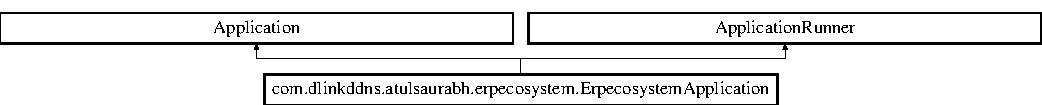
\includegraphics[height=1.407035cm]{classcom_1_1dlinkddns_1_1atulsaurabh_1_1erpecosystem_1_1_erpecosystem_application}
\end{center}
\end{figure}
\subsection*{Public Member Functions}
\begin{DoxyCompactItemize}
\item 
void \mbox{\hyperlink{classcom_1_1dlinkddns_1_1atulsaurabh_1_1erpecosystem_1_1_erpecosystem_application_a90a76d5aca54f84a9873a8121d3d0fad}{start}} (Stage primary\+Stage)  throws Exception 
\item 
void \mbox{\hyperlink{classcom_1_1dlinkddns_1_1atulsaurabh_1_1erpecosystem_1_1_erpecosystem_application_a440135636cc3274c5f73d337de252c6d}{run}} (Application\+Arguments args)  throws Exception 
\end{DoxyCompactItemize}
\subsection*{Static Public Member Functions}
\begin{DoxyCompactItemize}
\item 
static void \mbox{\hyperlink{classcom_1_1dlinkddns_1_1atulsaurabh_1_1erpecosystem_1_1_erpecosystem_application_a093269f7aa35ba687eaf9da0383564ab}{main}} (String\mbox{[}$\,$\mbox{]} args)
\end{DoxyCompactItemize}


\subsection{Detailed Description}


Definition at line 16 of file Erpecosystem\+Application.\+java.



\subsection{Member Function Documentation}
\mbox{\Hypertarget{classcom_1_1dlinkddns_1_1atulsaurabh_1_1erpecosystem_1_1_erpecosystem_application_a093269f7aa35ba687eaf9da0383564ab}\label{classcom_1_1dlinkddns_1_1atulsaurabh_1_1erpecosystem_1_1_erpecosystem_application_a093269f7aa35ba687eaf9da0383564ab}} 
\index{com\+::dlinkddns\+::atulsaurabh\+::erpecosystem\+::\+Erpecosystem\+Application@{com\+::dlinkddns\+::atulsaurabh\+::erpecosystem\+::\+Erpecosystem\+Application}!main@{main}}
\index{main@{main}!com\+::dlinkddns\+::atulsaurabh\+::erpecosystem\+::\+Erpecosystem\+Application@{com\+::dlinkddns\+::atulsaurabh\+::erpecosystem\+::\+Erpecosystem\+Application}}
\subsubsection{\texorpdfstring{main()}{main()}}
{\footnotesize\ttfamily static void com.\+dlinkddns.\+atulsaurabh.\+erpecosystem.\+Erpecosystem\+Application.\+main (\begin{DoxyParamCaption}\item[{String \mbox{[}$\,$\mbox{]}}]{args }\end{DoxyParamCaption})\hspace{0.3cm}{\ttfamily [static]}}



Definition at line 20 of file Erpecosystem\+Application.\+java.

\mbox{\Hypertarget{classcom_1_1dlinkddns_1_1atulsaurabh_1_1erpecosystem_1_1_erpecosystem_application_a440135636cc3274c5f73d337de252c6d}\label{classcom_1_1dlinkddns_1_1atulsaurabh_1_1erpecosystem_1_1_erpecosystem_application_a440135636cc3274c5f73d337de252c6d}} 
\index{com\+::dlinkddns\+::atulsaurabh\+::erpecosystem\+::\+Erpecosystem\+Application@{com\+::dlinkddns\+::atulsaurabh\+::erpecosystem\+::\+Erpecosystem\+Application}!run@{run}}
\index{run@{run}!com\+::dlinkddns\+::atulsaurabh\+::erpecosystem\+::\+Erpecosystem\+Application@{com\+::dlinkddns\+::atulsaurabh\+::erpecosystem\+::\+Erpecosystem\+Application}}
\subsubsection{\texorpdfstring{run()}{run()}}
{\footnotesize\ttfamily void com.\+dlinkddns.\+atulsaurabh.\+erpecosystem.\+Erpecosystem\+Application.\+run (\begin{DoxyParamCaption}\item[{Application\+Arguments}]{args }\end{DoxyParamCaption}) throws Exception}



Definition at line 52 of file Erpecosystem\+Application.\+java.

\mbox{\Hypertarget{classcom_1_1dlinkddns_1_1atulsaurabh_1_1erpecosystem_1_1_erpecosystem_application_a90a76d5aca54f84a9873a8121d3d0fad}\label{classcom_1_1dlinkddns_1_1atulsaurabh_1_1erpecosystem_1_1_erpecosystem_application_a90a76d5aca54f84a9873a8121d3d0fad}} 
\index{com\+::dlinkddns\+::atulsaurabh\+::erpecosystem\+::\+Erpecosystem\+Application@{com\+::dlinkddns\+::atulsaurabh\+::erpecosystem\+::\+Erpecosystem\+Application}!start@{start}}
\index{start@{start}!com\+::dlinkddns\+::atulsaurabh\+::erpecosystem\+::\+Erpecosystem\+Application@{com\+::dlinkddns\+::atulsaurabh\+::erpecosystem\+::\+Erpecosystem\+Application}}
\subsubsection{\texorpdfstring{start()}{start()}}
{\footnotesize\ttfamily void com.\+dlinkddns.\+atulsaurabh.\+erpecosystem.\+Erpecosystem\+Application.\+start (\begin{DoxyParamCaption}\item[{Stage}]{primary\+Stage }\end{DoxyParamCaption}) throws Exception}



Definition at line 25 of file Erpecosystem\+Application.\+java.



The documentation for this class was generated from the following file\+:\begin{DoxyCompactItemize}
\item 
C\+:/myworkplace/projects/erpecosystem/src/main/java/com/dlinkddns/atulsaurabh/erpecosystem/\mbox{\hyperlink{_erpecosystem_application_8java}{Erpecosystem\+Application.\+java}}\end{DoxyCompactItemize}

\hypertarget{classcom_1_1dlinkddns_1_1atulsaurabh_1_1erpecosystem_1_1logger_1_1_erp_ecosystem_logger}{}\section{com.\+dlinkddns.\+atulsaurabh.\+erpecosystem.\+logger.\+Erp\+Ecosystem\+Logger Class Reference}
\label{classcom_1_1dlinkddns_1_1atulsaurabh_1_1erpecosystem_1_1logger_1_1_erp_ecosystem_logger}\index{com.\+dlinkddns.\+atulsaurabh.\+erpecosystem.\+logger.\+Erp\+Ecosystem\+Logger@{com.\+dlinkddns.\+atulsaurabh.\+erpecosystem.\+logger.\+Erp\+Ecosystem\+Logger}}
Inheritance diagram for com.\+dlinkddns.\+atulsaurabh.\+erpecosystem.\+logger.\+Erp\+Ecosystem\+Logger\+:\begin{figure}[H]
\begin{center}
\leavevmode
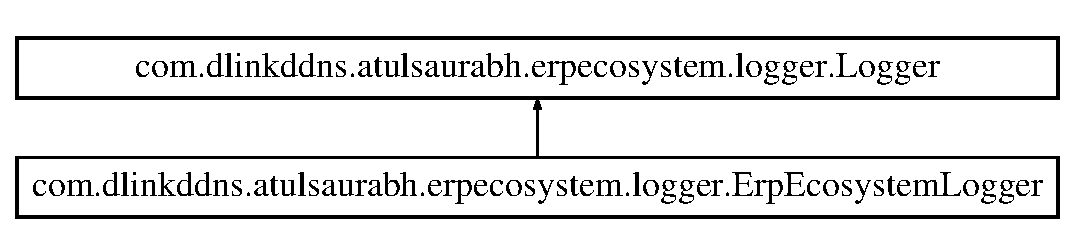
\includegraphics[height=2.000000cm]{classcom_1_1dlinkddns_1_1atulsaurabh_1_1erpecosystem_1_1logger_1_1_erp_ecosystem_logger}
\end{center}
\end{figure}
\subsection*{Public Member Functions}
\begin{DoxyCompactItemize}
\item 
void \mbox{\hyperlink{classcom_1_1dlinkddns_1_1atulsaurabh_1_1erpecosystem_1_1logger_1_1_erp_ecosystem_logger_a366c4448e35274f7b1edec8112fb2553}{log\+Fatal}} (String message)
\item 
void \mbox{\hyperlink{classcom_1_1dlinkddns_1_1atulsaurabh_1_1erpecosystem_1_1logger_1_1_erp_ecosystem_logger_ae9010d95c151f9940d3c4bcbb9a2f4b1}{log\+Fatal}} (Class error\+Class, String message)
\item 
void \mbox{\hyperlink{classcom_1_1dlinkddns_1_1atulsaurabh_1_1erpecosystem_1_1logger_1_1_erp_ecosystem_logger_a3def664f09892d36bbff6343fa8f3d6f}{log\+Fatal}} (Class error\+Class, String message, Throwable throwable)
\item 
void \mbox{\hyperlink{classcom_1_1dlinkddns_1_1atulsaurabh_1_1erpecosystem_1_1logger_1_1_erp_ecosystem_logger_a360f98d9c9cf93c49fbb0a6a1e3e922f}{log\+All}} (String message)
\item 
void \mbox{\hyperlink{classcom_1_1dlinkddns_1_1atulsaurabh_1_1erpecosystem_1_1logger_1_1_erp_ecosystem_logger_a5bea48485386781a9eee8a78c2e2c9be}{log\+All}} (Class error\+Class, String message)
\item 
void \mbox{\hyperlink{classcom_1_1dlinkddns_1_1atulsaurabh_1_1erpecosystem_1_1logger_1_1_erp_ecosystem_logger_a2706d4afe3cf3f8dad301d43851181ce}{log\+All}} (Class error\+Class, String message, Throwable throwable)
\item 
String \mbox{\hyperlink{classcom_1_1dlinkddns_1_1atulsaurabh_1_1erpecosystem_1_1logger_1_1_erp_ecosystem_logger_a8f0373f6917c8fe5a3ddea2c2adf081c}{get\+Conversion\+Pattern}} ()
\item 
void \mbox{\hyperlink{classcom_1_1dlinkddns_1_1atulsaurabh_1_1erpecosystem_1_1logger_1_1_erp_ecosystem_logger_a16d43ce13e22b9fae1b9e3b55a086b06}{set\+Conversion\+Pattern}} (String conversion\+Pattern)
\item 
void \mbox{\hyperlink{classcom_1_1dlinkddns_1_1atulsaurabh_1_1erpecosystem_1_1logger_1_1_erp_ecosystem_logger_a4a4c244511da1da97773a5a7933552d2}{log\+Warning}} (String message)
\item 
void \mbox{\hyperlink{classcom_1_1dlinkddns_1_1atulsaurabh_1_1erpecosystem_1_1logger_1_1_erp_ecosystem_logger_a7f8550d69fe0f6062f80c0cda4c74d87}{log\+Warning}} (Class warning\+Class, String message)
\item 
void \mbox{\hyperlink{classcom_1_1dlinkddns_1_1atulsaurabh_1_1erpecosystem_1_1logger_1_1_erp_ecosystem_logger_a432114edc56c223b7b5764348641ea24}{log\+Warning}} (Class warning\+Class, String message, Throwable throwable)
\item 
void \mbox{\hyperlink{classcom_1_1dlinkddns_1_1atulsaurabh_1_1erpecosystem_1_1logger_1_1_erp_ecosystem_logger_a25071d05590b133a88f8b2f35092ebd7}{log\+Info}} (String message)
\item 
void \mbox{\hyperlink{classcom_1_1dlinkddns_1_1atulsaurabh_1_1erpecosystem_1_1logger_1_1_erp_ecosystem_logger_a70838215b194b2f9771cec61a7f660c0}{log\+Info}} (Class info\+Class, String message)
\item 
void \mbox{\hyperlink{classcom_1_1dlinkddns_1_1atulsaurabh_1_1erpecosystem_1_1logger_1_1_erp_ecosystem_logger_ad6718b3031cb8032127659aeac49d803}{log\+Info}} (Class info\+Class, String message, Throwable throwable)
\item 
void \mbox{\hyperlink{classcom_1_1dlinkddns_1_1atulsaurabh_1_1erpecosystem_1_1logger_1_1_erp_ecosystem_logger_a220bd030f8fe67c986972c3925727196}{log\+Debug}} (String message)
\item 
void \mbox{\hyperlink{classcom_1_1dlinkddns_1_1atulsaurabh_1_1erpecosystem_1_1logger_1_1_erp_ecosystem_logger_a80d54c08b8d233dc1782e1f85bdde19a}{log\+Debug}} (Class debug\+Class, String message)
\item 
void \mbox{\hyperlink{classcom_1_1dlinkddns_1_1atulsaurabh_1_1erpecosystem_1_1logger_1_1_erp_ecosystem_logger_a40e19afc6e72a31339e4eec00132c166}{log\+Debug}} (Class debug\+Class, String message, Throwable throwable)
\item 
void \mbox{\hyperlink{classcom_1_1dlinkddns_1_1atulsaurabh_1_1erpecosystem_1_1logger_1_1_erp_ecosystem_logger_ab9553bd3b9e717accdc9c2d0ee13371e}{log\+Error}} (String message)
\item 
void \mbox{\hyperlink{classcom_1_1dlinkddns_1_1atulsaurabh_1_1erpecosystem_1_1logger_1_1_erp_ecosystem_logger_aa561000b385ff39f9d8171a91e831c2d}{log\+Error}} (Class error\+Class, String message)
\item 
void \mbox{\hyperlink{classcom_1_1dlinkddns_1_1atulsaurabh_1_1erpecosystem_1_1logger_1_1_erp_ecosystem_logger_a25316b3eabb66eaecba45d638c420b2b}{log\+Error}} (Class error\+Class, String message, Throwable throwable)
\end{DoxyCompactItemize}


\subsection{Detailed Description}
\paragraph*{Dependencies}

This implementation is depending upon \href{https://logging.apache.org/log4j/}{\tt Log4j}. To use this class in \href{https://maven.apache.org/}{\tt Maven} project following dependency need to added in the pom file. 
\begin{DoxyPre}

\begin{DoxyCode}
<dependency>
<groupId>log4j</groupId>
<artifactId>log4j</artifactId>
<version>1.2.17</version>
</dependency>
\end{DoxyCode}
 
 \end{DoxyPre}
 Otherwise Log4j dependencies need to be satisfied manually. \paragraph*{Purposes}

Purpose of this class is to provide a hassle free logging technique. The implementation supports rolling based logging as well as non rolling based logging mechanism. The rolling option can be activated by setting \mbox{\hyperlink{}{rolling\+On}} field.

Using this class following level of log can be recorded 
\begin{DoxyPre}
 \mbox{\hyperlink{}{org.apache.log4j.Level#ALL}}, \mbox{\hyperlink{}{org.apache.log4j.Level#DEBUG}},
 \mbox{\hyperlink{}{org.apache.log4j.Level#ERROR}}, \mbox{\hyperlink{}{org.apache.log4j.Level#FATAL}},
 \mbox{\hyperlink{}{org.apache.log4j.Level#INFO}} and \mbox{\hyperlink{}{org.apache.log4j.Level#WARN}}
 \end{DoxyPre}


\paragraph*{Configuration}

On the basis of above mentioned \mbox{\hyperlink{}{org.\+apache.\+log4j.\+Level}} and if the rolling is active then different type of log is recorded in different files. These files can be configured by changing inside {\bfseries application.\+properties} file. The following keys are used to configure the log files\+: 
\begin{DoxyItemize}
\item erp.\+log.\+alllogfilename \+: To log \mbox{\hyperlink{}{org.\+apache.\+log4j.\+Level\#\+A\+LL}} 
\item erp.\+log.\+debuflogfilename \+: To log \mbox{\hyperlink{}{org.\+apache.\+log4j.\+Level\#\+D\+E\+B\+UG}} 
\item erp.\+log.\+errorlogfilename \+: To log \mbox{\hyperlink{}{org.\+apache.\+log4j.\+Level\#\+E\+R\+R\+OR}} 
\item erp.\+log.\+fatallogfilename \+: To log \mbox{\hyperlink{}{org.\+apache.\+log4j.\+Level\#\+F\+A\+T\+AL}} 
\item erp.\+log.\+infologfilename \+: To log \mbox{\hyperlink{}{org.\+apache.\+log4j.\+Level\#\+I\+N\+FO}} 
\item erp.\+log.\+warnlogfilename \+: To log \mbox{\hyperlink{}{org.\+apache.\+log4j.\+Level\#\+W\+A\+RN}} 
\end{DoxyItemize}Along with the files, the director for log repository can also be configured by setting the key {\bfseries {\itshape erp.\+log.\+directory}} in application.\+properties file. \paragraph*{Features}

The rolling based logging mechanism provides a way to log the message on the basis of date and time. The date and time option is configurable. The format can be decided using \mbox{\hyperlink{}{date\+Pattern}}. 

The format of content is also configurable. This format can be modified using \mbox{\hyperlink{}{conversion\+Pattern}}

\begin{DoxySeeAlso}{See also}
\mbox{\hyperlink{interfacecom_1_1dlinkddns_1_1atulsaurabh_1_1erpecosystem_1_1logger_1_1_logger_af32bfcb68d536836f7bdb8618e4c1812}{set\+Rolling\+On(boolean)}} 

\mbox{\hyperlink{interfacecom_1_1dlinkddns_1_1atulsaurabh_1_1erpecosystem_1_1logger_1_1_logger_aceef18a85b09966b1ccf10c9927d0917}{set\+Date\+Pattern}}(java.\+lang.\+String) 

\mbox{\hyperlink{classcom_1_1dlinkddns_1_1atulsaurabh_1_1erpecosystem_1_1logger_1_1_erp_ecosystem_logger_a16d43ce13e22b9fae1b9e3b55a086b06}{set\+Conversion\+Pattern}}(java.\+lang.\+String)
\end{DoxySeeAlso}
\begin{DoxyVersion}{Version}
1.\+0 
\end{DoxyVersion}
\begin{DoxyAuthor}{Author}
Atul Saurabh 
\end{DoxyAuthor}
\begin{DoxySince}{Since}
1.\+0 
\end{DoxySince}


Definition at line 83 of file Erp\+Ecosystem\+Logger.\+java.



\subsection{Member Function Documentation}
\mbox{\Hypertarget{classcom_1_1dlinkddns_1_1atulsaurabh_1_1erpecosystem_1_1logger_1_1_erp_ecosystem_logger_a8f0373f6917c8fe5a3ddea2c2adf081c}\label{classcom_1_1dlinkddns_1_1atulsaurabh_1_1erpecosystem_1_1logger_1_1_erp_ecosystem_logger_a8f0373f6917c8fe5a3ddea2c2adf081c}} 
\index{com\+::dlinkddns\+::atulsaurabh\+::erpecosystem\+::logger\+::\+Erp\+Ecosystem\+Logger@{com\+::dlinkddns\+::atulsaurabh\+::erpecosystem\+::logger\+::\+Erp\+Ecosystem\+Logger}!get\+Conversion\+Pattern@{get\+Conversion\+Pattern}}
\index{get\+Conversion\+Pattern@{get\+Conversion\+Pattern}!com\+::dlinkddns\+::atulsaurabh\+::erpecosystem\+::logger\+::\+Erp\+Ecosystem\+Logger@{com\+::dlinkddns\+::atulsaurabh\+::erpecosystem\+::logger\+::\+Erp\+Ecosystem\+Logger}}
\subsubsection{\texorpdfstring{get\+Conversion\+Pattern()}{getConversionPattern()}}
{\footnotesize\ttfamily String com.\+dlinkddns.\+atulsaurabh.\+erpecosystem.\+logger.\+Erp\+Ecosystem\+Logger.\+get\+Conversion\+Pattern (\begin{DoxyParamCaption}{ }\end{DoxyParamCaption})}

\begin{DoxyReturn}{Returns}
Format for printing message into log file 
\end{DoxyReturn}


Implements \mbox{\hyperlink{interfacecom_1_1dlinkddns_1_1atulsaurabh_1_1erpecosystem_1_1logger_1_1_logger_ab9bd1ad5fb48fa4e46fb67fbbe2475f7}{com.\+dlinkddns.\+atulsaurabh.\+erpecosystem.\+logger.\+Logger}}.



Definition at line 281 of file Erp\+Ecosystem\+Logger.\+java.

\mbox{\Hypertarget{classcom_1_1dlinkddns_1_1atulsaurabh_1_1erpecosystem_1_1logger_1_1_erp_ecosystem_logger_a360f98d9c9cf93c49fbb0a6a1e3e922f}\label{classcom_1_1dlinkddns_1_1atulsaurabh_1_1erpecosystem_1_1logger_1_1_erp_ecosystem_logger_a360f98d9c9cf93c49fbb0a6a1e3e922f}} 
\index{com\+::dlinkddns\+::atulsaurabh\+::erpecosystem\+::logger\+::\+Erp\+Ecosystem\+Logger@{com\+::dlinkddns\+::atulsaurabh\+::erpecosystem\+::logger\+::\+Erp\+Ecosystem\+Logger}!log\+All@{log\+All}}
\index{log\+All@{log\+All}!com\+::dlinkddns\+::atulsaurabh\+::erpecosystem\+::logger\+::\+Erp\+Ecosystem\+Logger@{com\+::dlinkddns\+::atulsaurabh\+::erpecosystem\+::logger\+::\+Erp\+Ecosystem\+Logger}}
\subsubsection{\texorpdfstring{log\+All()}{logAll()}\hspace{0.1cm}{\footnotesize\ttfamily [1/3]}}
{\footnotesize\ttfamily void com.\+dlinkddns.\+atulsaurabh.\+erpecosystem.\+logger.\+Erp\+Ecosystem\+Logger.\+log\+All (\begin{DoxyParamCaption}\item[{String}]{message }\end{DoxyParamCaption})}


\begin{DoxyParams}{Parameters}
{\em message} & The message to be logged in. The logging will be done for every level. \\
\hline
\end{DoxyParams}


Implements \mbox{\hyperlink{interfacecom_1_1dlinkddns_1_1atulsaurabh_1_1erpecosystem_1_1logger_1_1_logger_a45d119fc284eee3233ca247ec5f92e4c}{com.\+dlinkddns.\+atulsaurabh.\+erpecosystem.\+logger.\+Logger}}.



Definition at line 161 of file Erp\+Ecosystem\+Logger.\+java.

\mbox{\Hypertarget{classcom_1_1dlinkddns_1_1atulsaurabh_1_1erpecosystem_1_1logger_1_1_erp_ecosystem_logger_a5bea48485386781a9eee8a78c2e2c9be}\label{classcom_1_1dlinkddns_1_1atulsaurabh_1_1erpecosystem_1_1logger_1_1_erp_ecosystem_logger_a5bea48485386781a9eee8a78c2e2c9be}} 
\index{com\+::dlinkddns\+::atulsaurabh\+::erpecosystem\+::logger\+::\+Erp\+Ecosystem\+Logger@{com\+::dlinkddns\+::atulsaurabh\+::erpecosystem\+::logger\+::\+Erp\+Ecosystem\+Logger}!log\+All@{log\+All}}
\index{log\+All@{log\+All}!com\+::dlinkddns\+::atulsaurabh\+::erpecosystem\+::logger\+::\+Erp\+Ecosystem\+Logger@{com\+::dlinkddns\+::atulsaurabh\+::erpecosystem\+::logger\+::\+Erp\+Ecosystem\+Logger}}
\subsubsection{\texorpdfstring{log\+All()}{logAll()}\hspace{0.1cm}{\footnotesize\ttfamily [2/3]}}
{\footnotesize\ttfamily void com.\+dlinkddns.\+atulsaurabh.\+erpecosystem.\+logger.\+Erp\+Ecosystem\+Logger.\+log\+All (\begin{DoxyParamCaption}\item[{Class}]{error\+Class,  }\item[{String}]{message }\end{DoxyParamCaption})}


\begin{DoxyParams}{Parameters}
{\em error\+Class} & The class where exception is caught \\
\hline
{\em message} & The message to be logged in. The logging will be done for every level. \\
\hline
\end{DoxyParams}


Implements \mbox{\hyperlink{interfacecom_1_1dlinkddns_1_1atulsaurabh_1_1erpecosystem_1_1logger_1_1_logger_a232415e10e9da278b0bacf82309aef76}{com.\+dlinkddns.\+atulsaurabh.\+erpecosystem.\+logger.\+Logger}}.



Definition at line 175 of file Erp\+Ecosystem\+Logger.\+java.

\mbox{\Hypertarget{classcom_1_1dlinkddns_1_1atulsaurabh_1_1erpecosystem_1_1logger_1_1_erp_ecosystem_logger_a2706d4afe3cf3f8dad301d43851181ce}\label{classcom_1_1dlinkddns_1_1atulsaurabh_1_1erpecosystem_1_1logger_1_1_erp_ecosystem_logger_a2706d4afe3cf3f8dad301d43851181ce}} 
\index{com\+::dlinkddns\+::atulsaurabh\+::erpecosystem\+::logger\+::\+Erp\+Ecosystem\+Logger@{com\+::dlinkddns\+::atulsaurabh\+::erpecosystem\+::logger\+::\+Erp\+Ecosystem\+Logger}!log\+All@{log\+All}}
\index{log\+All@{log\+All}!com\+::dlinkddns\+::atulsaurabh\+::erpecosystem\+::logger\+::\+Erp\+Ecosystem\+Logger@{com\+::dlinkddns\+::atulsaurabh\+::erpecosystem\+::logger\+::\+Erp\+Ecosystem\+Logger}}
\subsubsection{\texorpdfstring{log\+All()}{logAll()}\hspace{0.1cm}{\footnotesize\ttfamily [3/3]}}
{\footnotesize\ttfamily void com.\+dlinkddns.\+atulsaurabh.\+erpecosystem.\+logger.\+Erp\+Ecosystem\+Logger.\+log\+All (\begin{DoxyParamCaption}\item[{Class}]{error\+Class,  }\item[{String}]{message,  }\item[{Throwable}]{throwable }\end{DoxyParamCaption})}


\begin{DoxyParams}{Parameters}
{\em error\+Class} & The class where the exception is caught \\
\hline
{\em message} & The message to be logged in. The logging will be done for every level. \\
\hline
{\em throwable} & The exception generated. \\
\hline
\end{DoxyParams}


Implements \mbox{\hyperlink{interfacecom_1_1dlinkddns_1_1atulsaurabh_1_1erpecosystem_1_1logger_1_1_logger_aba1204d7d2383973ddf63e537e11086d}{com.\+dlinkddns.\+atulsaurabh.\+erpecosystem.\+logger.\+Logger}}.



Definition at line 189 of file Erp\+Ecosystem\+Logger.\+java.

\mbox{\Hypertarget{classcom_1_1dlinkddns_1_1atulsaurabh_1_1erpecosystem_1_1logger_1_1_erp_ecosystem_logger_a220bd030f8fe67c986972c3925727196}\label{classcom_1_1dlinkddns_1_1atulsaurabh_1_1erpecosystem_1_1logger_1_1_erp_ecosystem_logger_a220bd030f8fe67c986972c3925727196}} 
\index{com\+::dlinkddns\+::atulsaurabh\+::erpecosystem\+::logger\+::\+Erp\+Ecosystem\+Logger@{com\+::dlinkddns\+::atulsaurabh\+::erpecosystem\+::logger\+::\+Erp\+Ecosystem\+Logger}!log\+Debug@{log\+Debug}}
\index{log\+Debug@{log\+Debug}!com\+::dlinkddns\+::atulsaurabh\+::erpecosystem\+::logger\+::\+Erp\+Ecosystem\+Logger@{com\+::dlinkddns\+::atulsaurabh\+::erpecosystem\+::logger\+::\+Erp\+Ecosystem\+Logger}}
\subsubsection{\texorpdfstring{log\+Debug()}{logDebug()}\hspace{0.1cm}{\footnotesize\ttfamily [1/3]}}
{\footnotesize\ttfamily void com.\+dlinkddns.\+atulsaurabh.\+erpecosystem.\+logger.\+Erp\+Ecosystem\+Logger.\+log\+Debug (\begin{DoxyParamCaption}\item[{String}]{message }\end{DoxyParamCaption})}



Implements \mbox{\hyperlink{interfacecom_1_1dlinkddns_1_1atulsaurabh_1_1erpecosystem_1_1logger_1_1_logger_add9d87ff18f2b432002e2146b67b0f07}{com.\+dlinkddns.\+atulsaurabh.\+erpecosystem.\+logger.\+Logger}}.



Definition at line 331 of file Erp\+Ecosystem\+Logger.\+java.

\mbox{\Hypertarget{classcom_1_1dlinkddns_1_1atulsaurabh_1_1erpecosystem_1_1logger_1_1_erp_ecosystem_logger_a80d54c08b8d233dc1782e1f85bdde19a}\label{classcom_1_1dlinkddns_1_1atulsaurabh_1_1erpecosystem_1_1logger_1_1_erp_ecosystem_logger_a80d54c08b8d233dc1782e1f85bdde19a}} 
\index{com\+::dlinkddns\+::atulsaurabh\+::erpecosystem\+::logger\+::\+Erp\+Ecosystem\+Logger@{com\+::dlinkddns\+::atulsaurabh\+::erpecosystem\+::logger\+::\+Erp\+Ecosystem\+Logger}!log\+Debug@{log\+Debug}}
\index{log\+Debug@{log\+Debug}!com\+::dlinkddns\+::atulsaurabh\+::erpecosystem\+::logger\+::\+Erp\+Ecosystem\+Logger@{com\+::dlinkddns\+::atulsaurabh\+::erpecosystem\+::logger\+::\+Erp\+Ecosystem\+Logger}}
\subsubsection{\texorpdfstring{log\+Debug()}{logDebug()}\hspace{0.1cm}{\footnotesize\ttfamily [2/3]}}
{\footnotesize\ttfamily void com.\+dlinkddns.\+atulsaurabh.\+erpecosystem.\+logger.\+Erp\+Ecosystem\+Logger.\+log\+Debug (\begin{DoxyParamCaption}\item[{Class}]{debug\+Class,  }\item[{String}]{message }\end{DoxyParamCaption})}



Implements \mbox{\hyperlink{interfacecom_1_1dlinkddns_1_1atulsaurabh_1_1erpecosystem_1_1logger_1_1_logger_a8e94c010b6e08d96550a8ddc4b2f408e}{com.\+dlinkddns.\+atulsaurabh.\+erpecosystem.\+logger.\+Logger}}.



Definition at line 337 of file Erp\+Ecosystem\+Logger.\+java.

\mbox{\Hypertarget{classcom_1_1dlinkddns_1_1atulsaurabh_1_1erpecosystem_1_1logger_1_1_erp_ecosystem_logger_a40e19afc6e72a31339e4eec00132c166}\label{classcom_1_1dlinkddns_1_1atulsaurabh_1_1erpecosystem_1_1logger_1_1_erp_ecosystem_logger_a40e19afc6e72a31339e4eec00132c166}} 
\index{com\+::dlinkddns\+::atulsaurabh\+::erpecosystem\+::logger\+::\+Erp\+Ecosystem\+Logger@{com\+::dlinkddns\+::atulsaurabh\+::erpecosystem\+::logger\+::\+Erp\+Ecosystem\+Logger}!log\+Debug@{log\+Debug}}
\index{log\+Debug@{log\+Debug}!com\+::dlinkddns\+::atulsaurabh\+::erpecosystem\+::logger\+::\+Erp\+Ecosystem\+Logger@{com\+::dlinkddns\+::atulsaurabh\+::erpecosystem\+::logger\+::\+Erp\+Ecosystem\+Logger}}
\subsubsection{\texorpdfstring{log\+Debug()}{logDebug()}\hspace{0.1cm}{\footnotesize\ttfamily [3/3]}}
{\footnotesize\ttfamily void com.\+dlinkddns.\+atulsaurabh.\+erpecosystem.\+logger.\+Erp\+Ecosystem\+Logger.\+log\+Debug (\begin{DoxyParamCaption}\item[{Class}]{debug\+Class,  }\item[{String}]{message,  }\item[{Throwable}]{throwable }\end{DoxyParamCaption})}



Implements \mbox{\hyperlink{interfacecom_1_1dlinkddns_1_1atulsaurabh_1_1erpecosystem_1_1logger_1_1_logger_a95b44330997929adfe530e3c845e38f5}{com.\+dlinkddns.\+atulsaurabh.\+erpecosystem.\+logger.\+Logger}}.



Definition at line 343 of file Erp\+Ecosystem\+Logger.\+java.

\mbox{\Hypertarget{classcom_1_1dlinkddns_1_1atulsaurabh_1_1erpecosystem_1_1logger_1_1_erp_ecosystem_logger_ab9553bd3b9e717accdc9c2d0ee13371e}\label{classcom_1_1dlinkddns_1_1atulsaurabh_1_1erpecosystem_1_1logger_1_1_erp_ecosystem_logger_ab9553bd3b9e717accdc9c2d0ee13371e}} 
\index{com\+::dlinkddns\+::atulsaurabh\+::erpecosystem\+::logger\+::\+Erp\+Ecosystem\+Logger@{com\+::dlinkddns\+::atulsaurabh\+::erpecosystem\+::logger\+::\+Erp\+Ecosystem\+Logger}!log\+Error@{log\+Error}}
\index{log\+Error@{log\+Error}!com\+::dlinkddns\+::atulsaurabh\+::erpecosystem\+::logger\+::\+Erp\+Ecosystem\+Logger@{com\+::dlinkddns\+::atulsaurabh\+::erpecosystem\+::logger\+::\+Erp\+Ecosystem\+Logger}}
\subsubsection{\texorpdfstring{log\+Error()}{logError()}\hspace{0.1cm}{\footnotesize\ttfamily [1/3]}}
{\footnotesize\ttfamily void com.\+dlinkddns.\+atulsaurabh.\+erpecosystem.\+logger.\+Erp\+Ecosystem\+Logger.\+log\+Error (\begin{DoxyParamCaption}\item[{String}]{message }\end{DoxyParamCaption})}



Implements \mbox{\hyperlink{interfacecom_1_1dlinkddns_1_1atulsaurabh_1_1erpecosystem_1_1logger_1_1_logger_a0a9d496d0bbbd0afd87f13d38acb88e2}{com.\+dlinkddns.\+atulsaurabh.\+erpecosystem.\+logger.\+Logger}}.



Definition at line 349 of file Erp\+Ecosystem\+Logger.\+java.

\mbox{\Hypertarget{classcom_1_1dlinkddns_1_1atulsaurabh_1_1erpecosystem_1_1logger_1_1_erp_ecosystem_logger_aa561000b385ff39f9d8171a91e831c2d}\label{classcom_1_1dlinkddns_1_1atulsaurabh_1_1erpecosystem_1_1logger_1_1_erp_ecosystem_logger_aa561000b385ff39f9d8171a91e831c2d}} 
\index{com\+::dlinkddns\+::atulsaurabh\+::erpecosystem\+::logger\+::\+Erp\+Ecosystem\+Logger@{com\+::dlinkddns\+::atulsaurabh\+::erpecosystem\+::logger\+::\+Erp\+Ecosystem\+Logger}!log\+Error@{log\+Error}}
\index{log\+Error@{log\+Error}!com\+::dlinkddns\+::atulsaurabh\+::erpecosystem\+::logger\+::\+Erp\+Ecosystem\+Logger@{com\+::dlinkddns\+::atulsaurabh\+::erpecosystem\+::logger\+::\+Erp\+Ecosystem\+Logger}}
\subsubsection{\texorpdfstring{log\+Error()}{logError()}\hspace{0.1cm}{\footnotesize\ttfamily [2/3]}}
{\footnotesize\ttfamily void com.\+dlinkddns.\+atulsaurabh.\+erpecosystem.\+logger.\+Erp\+Ecosystem\+Logger.\+log\+Error (\begin{DoxyParamCaption}\item[{Class}]{error\+Class,  }\item[{String}]{message }\end{DoxyParamCaption})}



Implements \mbox{\hyperlink{interfacecom_1_1dlinkddns_1_1atulsaurabh_1_1erpecosystem_1_1logger_1_1_logger_a1cf0d549875c44c1afd8cd01dc0af1d6}{com.\+dlinkddns.\+atulsaurabh.\+erpecosystem.\+logger.\+Logger}}.



Definition at line 355 of file Erp\+Ecosystem\+Logger.\+java.

\mbox{\Hypertarget{classcom_1_1dlinkddns_1_1atulsaurabh_1_1erpecosystem_1_1logger_1_1_erp_ecosystem_logger_a25316b3eabb66eaecba45d638c420b2b}\label{classcom_1_1dlinkddns_1_1atulsaurabh_1_1erpecosystem_1_1logger_1_1_erp_ecosystem_logger_a25316b3eabb66eaecba45d638c420b2b}} 
\index{com\+::dlinkddns\+::atulsaurabh\+::erpecosystem\+::logger\+::\+Erp\+Ecosystem\+Logger@{com\+::dlinkddns\+::atulsaurabh\+::erpecosystem\+::logger\+::\+Erp\+Ecosystem\+Logger}!log\+Error@{log\+Error}}
\index{log\+Error@{log\+Error}!com\+::dlinkddns\+::atulsaurabh\+::erpecosystem\+::logger\+::\+Erp\+Ecosystem\+Logger@{com\+::dlinkddns\+::atulsaurabh\+::erpecosystem\+::logger\+::\+Erp\+Ecosystem\+Logger}}
\subsubsection{\texorpdfstring{log\+Error()}{logError()}\hspace{0.1cm}{\footnotesize\ttfamily [3/3]}}
{\footnotesize\ttfamily void com.\+dlinkddns.\+atulsaurabh.\+erpecosystem.\+logger.\+Erp\+Ecosystem\+Logger.\+log\+Error (\begin{DoxyParamCaption}\item[{Class}]{error\+Class,  }\item[{String}]{message,  }\item[{Throwable}]{throwable }\end{DoxyParamCaption})}



Implements \mbox{\hyperlink{interfacecom_1_1dlinkddns_1_1atulsaurabh_1_1erpecosystem_1_1logger_1_1_logger_a0f7488f980f029dfa98c465877b3fbe6}{com.\+dlinkddns.\+atulsaurabh.\+erpecosystem.\+logger.\+Logger}}.



Definition at line 361 of file Erp\+Ecosystem\+Logger.\+java.

\mbox{\Hypertarget{classcom_1_1dlinkddns_1_1atulsaurabh_1_1erpecosystem_1_1logger_1_1_erp_ecosystem_logger_a366c4448e35274f7b1edec8112fb2553}\label{classcom_1_1dlinkddns_1_1atulsaurabh_1_1erpecosystem_1_1logger_1_1_erp_ecosystem_logger_a366c4448e35274f7b1edec8112fb2553}} 
\index{com\+::dlinkddns\+::atulsaurabh\+::erpecosystem\+::logger\+::\+Erp\+Ecosystem\+Logger@{com\+::dlinkddns\+::atulsaurabh\+::erpecosystem\+::logger\+::\+Erp\+Ecosystem\+Logger}!log\+Fatal@{log\+Fatal}}
\index{log\+Fatal@{log\+Fatal}!com\+::dlinkddns\+::atulsaurabh\+::erpecosystem\+::logger\+::\+Erp\+Ecosystem\+Logger@{com\+::dlinkddns\+::atulsaurabh\+::erpecosystem\+::logger\+::\+Erp\+Ecosystem\+Logger}}
\subsubsection{\texorpdfstring{log\+Fatal()}{logFatal()}\hspace{0.1cm}{\footnotesize\ttfamily [1/3]}}
{\footnotesize\ttfamily void com.\+dlinkddns.\+atulsaurabh.\+erpecosystem.\+logger.\+Erp\+Ecosystem\+Logger.\+log\+Fatal (\begin{DoxyParamCaption}\item[{String}]{message }\end{DoxyParamCaption})}

Logs the fatal level. 
\begin{DoxyParams}{Parameters}
{\em message} & The fatal level message to be logged in \\
\hline
\end{DoxyParams}
\begin{DoxySince}{Since}
1.\+0 
\end{DoxySince}


Implements \mbox{\hyperlink{interfacecom_1_1dlinkddns_1_1atulsaurabh_1_1erpecosystem_1_1logger_1_1_logger_ab1796d8ce066433e34409055fd5e7100}{com.\+dlinkddns.\+atulsaurabh.\+erpecosystem.\+logger.\+Logger}}.



Definition at line 124 of file Erp\+Ecosystem\+Logger.\+java.

\mbox{\Hypertarget{classcom_1_1dlinkddns_1_1atulsaurabh_1_1erpecosystem_1_1logger_1_1_erp_ecosystem_logger_ae9010d95c151f9940d3c4bcbb9a2f4b1}\label{classcom_1_1dlinkddns_1_1atulsaurabh_1_1erpecosystem_1_1logger_1_1_erp_ecosystem_logger_ae9010d95c151f9940d3c4bcbb9a2f4b1}} 
\index{com\+::dlinkddns\+::atulsaurabh\+::erpecosystem\+::logger\+::\+Erp\+Ecosystem\+Logger@{com\+::dlinkddns\+::atulsaurabh\+::erpecosystem\+::logger\+::\+Erp\+Ecosystem\+Logger}!log\+Fatal@{log\+Fatal}}
\index{log\+Fatal@{log\+Fatal}!com\+::dlinkddns\+::atulsaurabh\+::erpecosystem\+::logger\+::\+Erp\+Ecosystem\+Logger@{com\+::dlinkddns\+::atulsaurabh\+::erpecosystem\+::logger\+::\+Erp\+Ecosystem\+Logger}}
\subsubsection{\texorpdfstring{log\+Fatal()}{logFatal()}\hspace{0.1cm}{\footnotesize\ttfamily [2/3]}}
{\footnotesize\ttfamily void com.\+dlinkddns.\+atulsaurabh.\+erpecosystem.\+logger.\+Erp\+Ecosystem\+Logger.\+log\+Fatal (\begin{DoxyParamCaption}\item[{Class}]{error\+Class,  }\item[{String}]{message }\end{DoxyParamCaption})}


\begin{DoxyParams}{Parameters}
{\em error\+Class} & The class where the exception is generated \\
\hline
{\em message} & The fatal level message to be logged in \\
\hline
\end{DoxyParams}


Implements \mbox{\hyperlink{interfacecom_1_1dlinkddns_1_1atulsaurabh_1_1erpecosystem_1_1logger_1_1_logger_ae9763257a2db31ecdfd4675bcdcd3bd0}{com.\+dlinkddns.\+atulsaurabh.\+erpecosystem.\+logger.\+Logger}}.



Definition at line 136 of file Erp\+Ecosystem\+Logger.\+java.

\mbox{\Hypertarget{classcom_1_1dlinkddns_1_1atulsaurabh_1_1erpecosystem_1_1logger_1_1_erp_ecosystem_logger_a3def664f09892d36bbff6343fa8f3d6f}\label{classcom_1_1dlinkddns_1_1atulsaurabh_1_1erpecosystem_1_1logger_1_1_erp_ecosystem_logger_a3def664f09892d36bbff6343fa8f3d6f}} 
\index{com\+::dlinkddns\+::atulsaurabh\+::erpecosystem\+::logger\+::\+Erp\+Ecosystem\+Logger@{com\+::dlinkddns\+::atulsaurabh\+::erpecosystem\+::logger\+::\+Erp\+Ecosystem\+Logger}!log\+Fatal@{log\+Fatal}}
\index{log\+Fatal@{log\+Fatal}!com\+::dlinkddns\+::atulsaurabh\+::erpecosystem\+::logger\+::\+Erp\+Ecosystem\+Logger@{com\+::dlinkddns\+::atulsaurabh\+::erpecosystem\+::logger\+::\+Erp\+Ecosystem\+Logger}}
\subsubsection{\texorpdfstring{log\+Fatal()}{logFatal()}\hspace{0.1cm}{\footnotesize\ttfamily [3/3]}}
{\footnotesize\ttfamily void com.\+dlinkddns.\+atulsaurabh.\+erpecosystem.\+logger.\+Erp\+Ecosystem\+Logger.\+log\+Fatal (\begin{DoxyParamCaption}\item[{Class}]{error\+Class,  }\item[{String}]{message,  }\item[{Throwable}]{throwable }\end{DoxyParamCaption})}


\begin{DoxyParams}{Parameters}
{\em error\+Class} & The class where the exception is generated \\
\hline
{\em message} & The fatal level message to be logged in \\
\hline
{\em throwable} & The exception to be logged in \\
\hline
\end{DoxyParams}


Implements \mbox{\hyperlink{interfacecom_1_1dlinkddns_1_1atulsaurabh_1_1erpecosystem_1_1logger_1_1_logger_ad8e4ea32b41f7d225b8ea824af177a43}{com.\+dlinkddns.\+atulsaurabh.\+erpecosystem.\+logger.\+Logger}}.



Definition at line 149 of file Erp\+Ecosystem\+Logger.\+java.

\mbox{\Hypertarget{classcom_1_1dlinkddns_1_1atulsaurabh_1_1erpecosystem_1_1logger_1_1_erp_ecosystem_logger_a25071d05590b133a88f8b2f35092ebd7}\label{classcom_1_1dlinkddns_1_1atulsaurabh_1_1erpecosystem_1_1logger_1_1_erp_ecosystem_logger_a25071d05590b133a88f8b2f35092ebd7}} 
\index{com\+::dlinkddns\+::atulsaurabh\+::erpecosystem\+::logger\+::\+Erp\+Ecosystem\+Logger@{com\+::dlinkddns\+::atulsaurabh\+::erpecosystem\+::logger\+::\+Erp\+Ecosystem\+Logger}!log\+Info@{log\+Info}}
\index{log\+Info@{log\+Info}!com\+::dlinkddns\+::atulsaurabh\+::erpecosystem\+::logger\+::\+Erp\+Ecosystem\+Logger@{com\+::dlinkddns\+::atulsaurabh\+::erpecosystem\+::logger\+::\+Erp\+Ecosystem\+Logger}}
\subsubsection{\texorpdfstring{log\+Info()}{logInfo()}\hspace{0.1cm}{\footnotesize\ttfamily [1/3]}}
{\footnotesize\ttfamily void com.\+dlinkddns.\+atulsaurabh.\+erpecosystem.\+logger.\+Erp\+Ecosystem\+Logger.\+log\+Info (\begin{DoxyParamCaption}\item[{String}]{message }\end{DoxyParamCaption})}



Implements \mbox{\hyperlink{interfacecom_1_1dlinkddns_1_1atulsaurabh_1_1erpecosystem_1_1logger_1_1_logger_a8671e0fd90d8f2fbb4024d7a73d9070d}{com.\+dlinkddns.\+atulsaurabh.\+erpecosystem.\+logger.\+Logger}}.



Definition at line 313 of file Erp\+Ecosystem\+Logger.\+java.

\mbox{\Hypertarget{classcom_1_1dlinkddns_1_1atulsaurabh_1_1erpecosystem_1_1logger_1_1_erp_ecosystem_logger_a70838215b194b2f9771cec61a7f660c0}\label{classcom_1_1dlinkddns_1_1atulsaurabh_1_1erpecosystem_1_1logger_1_1_erp_ecosystem_logger_a70838215b194b2f9771cec61a7f660c0}} 
\index{com\+::dlinkddns\+::atulsaurabh\+::erpecosystem\+::logger\+::\+Erp\+Ecosystem\+Logger@{com\+::dlinkddns\+::atulsaurabh\+::erpecosystem\+::logger\+::\+Erp\+Ecosystem\+Logger}!log\+Info@{log\+Info}}
\index{log\+Info@{log\+Info}!com\+::dlinkddns\+::atulsaurabh\+::erpecosystem\+::logger\+::\+Erp\+Ecosystem\+Logger@{com\+::dlinkddns\+::atulsaurabh\+::erpecosystem\+::logger\+::\+Erp\+Ecosystem\+Logger}}
\subsubsection{\texorpdfstring{log\+Info()}{logInfo()}\hspace{0.1cm}{\footnotesize\ttfamily [2/3]}}
{\footnotesize\ttfamily void com.\+dlinkddns.\+atulsaurabh.\+erpecosystem.\+logger.\+Erp\+Ecosystem\+Logger.\+log\+Info (\begin{DoxyParamCaption}\item[{Class}]{info\+Class,  }\item[{String}]{message }\end{DoxyParamCaption})}



Implements \mbox{\hyperlink{interfacecom_1_1dlinkddns_1_1atulsaurabh_1_1erpecosystem_1_1logger_1_1_logger_a37e8723a5243a845e140d2edb6d7f701}{com.\+dlinkddns.\+atulsaurabh.\+erpecosystem.\+logger.\+Logger}}.



Definition at line 319 of file Erp\+Ecosystem\+Logger.\+java.

\mbox{\Hypertarget{classcom_1_1dlinkddns_1_1atulsaurabh_1_1erpecosystem_1_1logger_1_1_erp_ecosystem_logger_ad6718b3031cb8032127659aeac49d803}\label{classcom_1_1dlinkddns_1_1atulsaurabh_1_1erpecosystem_1_1logger_1_1_erp_ecosystem_logger_ad6718b3031cb8032127659aeac49d803}} 
\index{com\+::dlinkddns\+::atulsaurabh\+::erpecosystem\+::logger\+::\+Erp\+Ecosystem\+Logger@{com\+::dlinkddns\+::atulsaurabh\+::erpecosystem\+::logger\+::\+Erp\+Ecosystem\+Logger}!log\+Info@{log\+Info}}
\index{log\+Info@{log\+Info}!com\+::dlinkddns\+::atulsaurabh\+::erpecosystem\+::logger\+::\+Erp\+Ecosystem\+Logger@{com\+::dlinkddns\+::atulsaurabh\+::erpecosystem\+::logger\+::\+Erp\+Ecosystem\+Logger}}
\subsubsection{\texorpdfstring{log\+Info()}{logInfo()}\hspace{0.1cm}{\footnotesize\ttfamily [3/3]}}
{\footnotesize\ttfamily void com.\+dlinkddns.\+atulsaurabh.\+erpecosystem.\+logger.\+Erp\+Ecosystem\+Logger.\+log\+Info (\begin{DoxyParamCaption}\item[{Class}]{info\+Class,  }\item[{String}]{message,  }\item[{Throwable}]{throwable }\end{DoxyParamCaption})}



Implements \mbox{\hyperlink{interfacecom_1_1dlinkddns_1_1atulsaurabh_1_1erpecosystem_1_1logger_1_1_logger_a0a674a1745e0f50d11b1f8be2c4d1726}{com.\+dlinkddns.\+atulsaurabh.\+erpecosystem.\+logger.\+Logger}}.



Definition at line 325 of file Erp\+Ecosystem\+Logger.\+java.

\mbox{\Hypertarget{classcom_1_1dlinkddns_1_1atulsaurabh_1_1erpecosystem_1_1logger_1_1_erp_ecosystem_logger_a4a4c244511da1da97773a5a7933552d2}\label{classcom_1_1dlinkddns_1_1atulsaurabh_1_1erpecosystem_1_1logger_1_1_erp_ecosystem_logger_a4a4c244511da1da97773a5a7933552d2}} 
\index{com\+::dlinkddns\+::atulsaurabh\+::erpecosystem\+::logger\+::\+Erp\+Ecosystem\+Logger@{com\+::dlinkddns\+::atulsaurabh\+::erpecosystem\+::logger\+::\+Erp\+Ecosystem\+Logger}!log\+Warning@{log\+Warning}}
\index{log\+Warning@{log\+Warning}!com\+::dlinkddns\+::atulsaurabh\+::erpecosystem\+::logger\+::\+Erp\+Ecosystem\+Logger@{com\+::dlinkddns\+::atulsaurabh\+::erpecosystem\+::logger\+::\+Erp\+Ecosystem\+Logger}}
\subsubsection{\texorpdfstring{log\+Warning()}{logWarning()}\hspace{0.1cm}{\footnotesize\ttfamily [1/3]}}
{\footnotesize\ttfamily void com.\+dlinkddns.\+atulsaurabh.\+erpecosystem.\+logger.\+Erp\+Ecosystem\+Logger.\+log\+Warning (\begin{DoxyParamCaption}\item[{String}]{message }\end{DoxyParamCaption})}



Implements \mbox{\hyperlink{interfacecom_1_1dlinkddns_1_1atulsaurabh_1_1erpecosystem_1_1logger_1_1_logger_aab8d04f52fde89ff5e58d84b40e25144}{com.\+dlinkddns.\+atulsaurabh.\+erpecosystem.\+logger.\+Logger}}.



Definition at line 295 of file Erp\+Ecosystem\+Logger.\+java.

\mbox{\Hypertarget{classcom_1_1dlinkddns_1_1atulsaurabh_1_1erpecosystem_1_1logger_1_1_erp_ecosystem_logger_a7f8550d69fe0f6062f80c0cda4c74d87}\label{classcom_1_1dlinkddns_1_1atulsaurabh_1_1erpecosystem_1_1logger_1_1_erp_ecosystem_logger_a7f8550d69fe0f6062f80c0cda4c74d87}} 
\index{com\+::dlinkddns\+::atulsaurabh\+::erpecosystem\+::logger\+::\+Erp\+Ecosystem\+Logger@{com\+::dlinkddns\+::atulsaurabh\+::erpecosystem\+::logger\+::\+Erp\+Ecosystem\+Logger}!log\+Warning@{log\+Warning}}
\index{log\+Warning@{log\+Warning}!com\+::dlinkddns\+::atulsaurabh\+::erpecosystem\+::logger\+::\+Erp\+Ecosystem\+Logger@{com\+::dlinkddns\+::atulsaurabh\+::erpecosystem\+::logger\+::\+Erp\+Ecosystem\+Logger}}
\subsubsection{\texorpdfstring{log\+Warning()}{logWarning()}\hspace{0.1cm}{\footnotesize\ttfamily [2/3]}}
{\footnotesize\ttfamily void com.\+dlinkddns.\+atulsaurabh.\+erpecosystem.\+logger.\+Erp\+Ecosystem\+Logger.\+log\+Warning (\begin{DoxyParamCaption}\item[{Class}]{warning\+Class,  }\item[{String}]{message }\end{DoxyParamCaption})}



Implements \mbox{\hyperlink{interfacecom_1_1dlinkddns_1_1atulsaurabh_1_1erpecosystem_1_1logger_1_1_logger_aa5df260afe6fcae92f5a9236b3b6a983}{com.\+dlinkddns.\+atulsaurabh.\+erpecosystem.\+logger.\+Logger}}.



Definition at line 301 of file Erp\+Ecosystem\+Logger.\+java.

\mbox{\Hypertarget{classcom_1_1dlinkddns_1_1atulsaurabh_1_1erpecosystem_1_1logger_1_1_erp_ecosystem_logger_a432114edc56c223b7b5764348641ea24}\label{classcom_1_1dlinkddns_1_1atulsaurabh_1_1erpecosystem_1_1logger_1_1_erp_ecosystem_logger_a432114edc56c223b7b5764348641ea24}} 
\index{com\+::dlinkddns\+::atulsaurabh\+::erpecosystem\+::logger\+::\+Erp\+Ecosystem\+Logger@{com\+::dlinkddns\+::atulsaurabh\+::erpecosystem\+::logger\+::\+Erp\+Ecosystem\+Logger}!log\+Warning@{log\+Warning}}
\index{log\+Warning@{log\+Warning}!com\+::dlinkddns\+::atulsaurabh\+::erpecosystem\+::logger\+::\+Erp\+Ecosystem\+Logger@{com\+::dlinkddns\+::atulsaurabh\+::erpecosystem\+::logger\+::\+Erp\+Ecosystem\+Logger}}
\subsubsection{\texorpdfstring{log\+Warning()}{logWarning()}\hspace{0.1cm}{\footnotesize\ttfamily [3/3]}}
{\footnotesize\ttfamily void com.\+dlinkddns.\+atulsaurabh.\+erpecosystem.\+logger.\+Erp\+Ecosystem\+Logger.\+log\+Warning (\begin{DoxyParamCaption}\item[{Class}]{warning\+Class,  }\item[{String}]{message,  }\item[{Throwable}]{throwable }\end{DoxyParamCaption})}



Implements \mbox{\hyperlink{interfacecom_1_1dlinkddns_1_1atulsaurabh_1_1erpecosystem_1_1logger_1_1_logger_a05aa52bed792e7a4a3519dadaab2f4f3}{com.\+dlinkddns.\+atulsaurabh.\+erpecosystem.\+logger.\+Logger}}.



Definition at line 307 of file Erp\+Ecosystem\+Logger.\+java.

\mbox{\Hypertarget{classcom_1_1dlinkddns_1_1atulsaurabh_1_1erpecosystem_1_1logger_1_1_erp_ecosystem_logger_a16d43ce13e22b9fae1b9e3b55a086b06}\label{classcom_1_1dlinkddns_1_1atulsaurabh_1_1erpecosystem_1_1logger_1_1_erp_ecosystem_logger_a16d43ce13e22b9fae1b9e3b55a086b06}} 
\index{com\+::dlinkddns\+::atulsaurabh\+::erpecosystem\+::logger\+::\+Erp\+Ecosystem\+Logger@{com\+::dlinkddns\+::atulsaurabh\+::erpecosystem\+::logger\+::\+Erp\+Ecosystem\+Logger}!set\+Conversion\+Pattern@{set\+Conversion\+Pattern}}
\index{set\+Conversion\+Pattern@{set\+Conversion\+Pattern}!com\+::dlinkddns\+::atulsaurabh\+::erpecosystem\+::logger\+::\+Erp\+Ecosystem\+Logger@{com\+::dlinkddns\+::atulsaurabh\+::erpecosystem\+::logger\+::\+Erp\+Ecosystem\+Logger}}
\subsubsection{\texorpdfstring{set\+Conversion\+Pattern()}{setConversionPattern()}}
{\footnotesize\ttfamily void com.\+dlinkddns.\+atulsaurabh.\+erpecosystem.\+logger.\+Erp\+Ecosystem\+Logger.\+set\+Conversion\+Pattern (\begin{DoxyParamCaption}\item[{String}]{pattern }\end{DoxyParamCaption})}


\begin{DoxyParams}{Parameters}
{\em pattern} & Format for printing message into log file \\
\hline
\end{DoxyParams}


Implements \mbox{\hyperlink{interfacecom_1_1dlinkddns_1_1atulsaurabh_1_1erpecosystem_1_1logger_1_1_logger_add9a38d7fa3907aa924bdfe56f3fe5c3}{com.\+dlinkddns.\+atulsaurabh.\+erpecosystem.\+logger.\+Logger}}.



Definition at line 290 of file Erp\+Ecosystem\+Logger.\+java.



The documentation for this class was generated from the following file\+:\begin{DoxyCompactItemize}
\item 
C\+:/myworkplace/projects/erpecosystem/src/main/java/com/dlinkddns/atulsaurabh/erpecosystem/logger/\mbox{\hyperlink{_erp_ecosystem_logger_8java}{Erp\+Ecosystem\+Logger.\+java}}\end{DoxyCompactItemize}

\hypertarget{interfacecom_1_1dlinkddns_1_1atulsaurabh_1_1erpecosystem_1_1util_1_1_erp_utility}{}\section{com.\+dlinkddns.\+atulsaurabh.\+erpecosystem.\+util.\+Erp\+Utility Interface Reference}
\label{interfacecom_1_1dlinkddns_1_1atulsaurabh_1_1erpecosystem_1_1util_1_1_erp_utility}\index{com.\+dlinkddns.\+atulsaurabh.\+erpecosystem.\+util.\+Erp\+Utility@{com.\+dlinkddns.\+atulsaurabh.\+erpecosystem.\+util.\+Erp\+Utility}}
Inheritance diagram for com.\+dlinkddns.\+atulsaurabh.\+erpecosystem.\+util.\+Erp\+Utility\+:\begin{figure}[H]
\begin{center}
\leavevmode
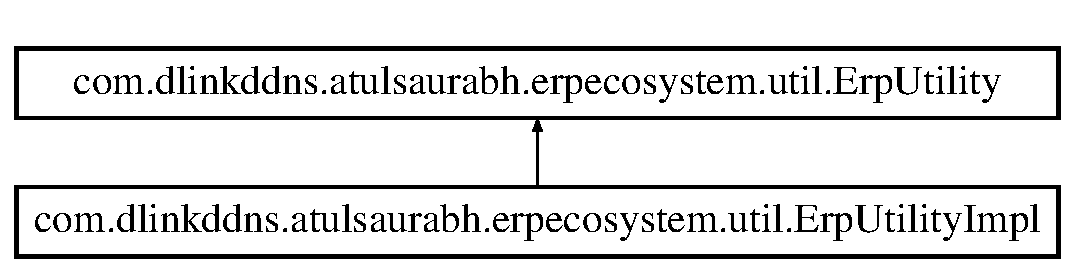
\includegraphics[height=2.000000cm]{interfacecom_1_1dlinkddns_1_1atulsaurabh_1_1erpecosystem_1_1util_1_1_erp_utility}
\end{center}
\end{figure}
\subsection*{Public Member Functions}
\begin{DoxyCompactItemize}
\item 
String \mbox{\hyperlink{interfacecom_1_1dlinkddns_1_1atulsaurabh_1_1erpecosystem_1_1util_1_1_erp_utility_a177b7a6f2a1ab3a9e620ca914ddcd6d9}{resolv\+Key}} (String key)
\end{DoxyCompactItemize}


\subsection{Detailed Description}
\begin{DoxyAuthor}{Author}
Suyojan 
\end{DoxyAuthor}


\subsection{Member Function Documentation}
\mbox{\Hypertarget{interfacecom_1_1dlinkddns_1_1atulsaurabh_1_1erpecosystem_1_1util_1_1_erp_utility_a177b7a6f2a1ab3a9e620ca914ddcd6d9}\label{interfacecom_1_1dlinkddns_1_1atulsaurabh_1_1erpecosystem_1_1util_1_1_erp_utility_a177b7a6f2a1ab3a9e620ca914ddcd6d9}} 
\index{com\+::dlinkddns\+::atulsaurabh\+::erpecosystem\+::util\+::\+Erp\+Utility@{com\+::dlinkddns\+::atulsaurabh\+::erpecosystem\+::util\+::\+Erp\+Utility}!resolv\+Key@{resolv\+Key}}
\index{resolv\+Key@{resolv\+Key}!com\+::dlinkddns\+::atulsaurabh\+::erpecosystem\+::util\+::\+Erp\+Utility@{com\+::dlinkddns\+::atulsaurabh\+::erpecosystem\+::util\+::\+Erp\+Utility}}
\subsubsection{\texorpdfstring{resolv\+Key()}{resolvKey()}}
{\footnotesize\ttfamily String com.\+dlinkddns.\+atulsaurabh.\+erpecosystem.\+util.\+Erp\+Utility.\+resolv\+Key (\begin{DoxyParamCaption}\item[{String}]{key }\end{DoxyParamCaption})}



Implemented in \mbox{\hyperlink{classcom_1_1dlinkddns_1_1atulsaurabh_1_1erpecosystem_1_1util_1_1_erp_utility_impl_af2cfed2c5aca189be0e160b0610f2644}{com.\+dlinkddns.\+atulsaurabh.\+erpecosystem.\+util.\+Erp\+Utility\+Impl}}.



The documentation for this interface was generated from the following file\+:\begin{DoxyCompactItemize}
\item 
com/dlinkddns/atulsaurabh/erpecosystem/util/\mbox{\hyperlink{_erp_utility_8java}{Erp\+Utility.\+java}}\end{DoxyCompactItemize}

\hypertarget{classcom_1_1dlinkddns_1_1atulsaurabh_1_1erpecosystem_1_1util_1_1_erp_utility_impl}{}\section{com.\+dlinkddns.\+atulsaurabh.\+erpecosystem.\+util.\+Erp\+Utility\+Impl Class Reference}
\label{classcom_1_1dlinkddns_1_1atulsaurabh_1_1erpecosystem_1_1util_1_1_erp_utility_impl}\index{com.\+dlinkddns.\+atulsaurabh.\+erpecosystem.\+util.\+Erp\+Utility\+Impl@{com.\+dlinkddns.\+atulsaurabh.\+erpecosystem.\+util.\+Erp\+Utility\+Impl}}
Inheritance diagram for com.\+dlinkddns.\+atulsaurabh.\+erpecosystem.\+util.\+Erp\+Utility\+Impl\+:\begin{figure}[H]
\begin{center}
\leavevmode
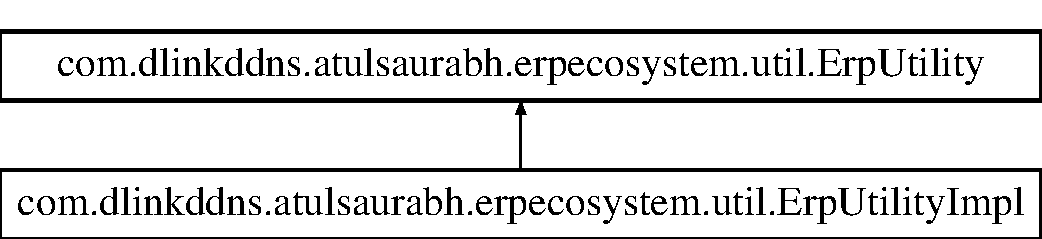
\includegraphics[height=2.000000cm]{classcom_1_1dlinkddns_1_1atulsaurabh_1_1erpecosystem_1_1util_1_1_erp_utility_impl}
\end{center}
\end{figure}
\subsection*{Public Member Functions}
\begin{DoxyCompactItemize}
\item 
String \mbox{\hyperlink{classcom_1_1dlinkddns_1_1atulsaurabh_1_1erpecosystem_1_1util_1_1_erp_utility_impl_af2cfed2c5aca189be0e160b0610f2644}{resolv\+Key}} (String key)
\end{DoxyCompactItemize}


\subsection{Detailed Description}
\begin{DoxyAuthor}{Author}
Atul Saurabh 
\end{DoxyAuthor}
\begin{DoxyVersion}{Version}
1.\+0 
\end{DoxyVersion}


Definition at line 16 of file Erp\+Utility\+Impl.\+java.



\subsection{Member Function Documentation}
\mbox{\Hypertarget{classcom_1_1dlinkddns_1_1atulsaurabh_1_1erpecosystem_1_1util_1_1_erp_utility_impl_af2cfed2c5aca189be0e160b0610f2644}\label{classcom_1_1dlinkddns_1_1atulsaurabh_1_1erpecosystem_1_1util_1_1_erp_utility_impl_af2cfed2c5aca189be0e160b0610f2644}} 
\index{com\+::dlinkddns\+::atulsaurabh\+::erpecosystem\+::util\+::\+Erp\+Utility\+Impl@{com\+::dlinkddns\+::atulsaurabh\+::erpecosystem\+::util\+::\+Erp\+Utility\+Impl}!resolv\+Key@{resolv\+Key}}
\index{resolv\+Key@{resolv\+Key}!com\+::dlinkddns\+::atulsaurabh\+::erpecosystem\+::util\+::\+Erp\+Utility\+Impl@{com\+::dlinkddns\+::atulsaurabh\+::erpecosystem\+::util\+::\+Erp\+Utility\+Impl}}
\subsubsection{\texorpdfstring{resolv\+Key()}{resolvKey()}}
{\footnotesize\ttfamily String com.\+dlinkddns.\+atulsaurabh.\+erpecosystem.\+util.\+Erp\+Utility\+Impl.\+resolv\+Key (\begin{DoxyParamCaption}\item[{String}]{key }\end{DoxyParamCaption})}



Implements \mbox{\hyperlink{interfacecom_1_1dlinkddns_1_1atulsaurabh_1_1erpecosystem_1_1util_1_1_erp_utility_a177b7a6f2a1ab3a9e620ca914ddcd6d9}{com.\+dlinkddns.\+atulsaurabh.\+erpecosystem.\+util.\+Erp\+Utility}}.



Definition at line 22 of file Erp\+Utility\+Impl.\+java.



The documentation for this class was generated from the following file\+:\begin{DoxyCompactItemize}
\item 
C\+:/myworkplace/projects/erpecosystem/src/main/java/com/dlinkddns/atulsaurabh/erpecosystem/util/\mbox{\hyperlink{_erp_utility_impl_8java}{Erp\+Utility\+Impl.\+java}}\end{DoxyCompactItemize}

\hypertarget{interfacecom_1_1dlinkddns_1_1atulsaurabh_1_1erpecosystem_1_1loader_1_1_g_u_i_info}{}\section{com.\+dlinkddns.\+atulsaurabh.\+erpecosystem.\+loader.\+G\+U\+I\+Info Interface Reference}
\label{interfacecom_1_1dlinkddns_1_1atulsaurabh_1_1erpecosystem_1_1loader_1_1_g_u_i_info}\index{com.\+dlinkddns.\+atulsaurabh.\+erpecosystem.\+loader.\+G\+U\+I\+Info@{com.\+dlinkddns.\+atulsaurabh.\+erpecosystem.\+loader.\+G\+U\+I\+Info}}
\subsection*{Static Public Attributes}
\begin{DoxyCompactItemize}
\item 
static final String \mbox{\hyperlink{interfacecom_1_1dlinkddns_1_1atulsaurabh_1_1erpecosystem_1_1loader_1_1_g_u_i_info_a9357425e3de4062e155fe1fff7f920be}{G\+U\+I\+\_\+\+H\+O\+ME}} =\char`\"{}/gui/\char`\"{}
\end{DoxyCompactItemize}


\subsection{Detailed Description}
\begin{DoxyAuthor}{Author}
Suyojan 
\end{DoxyAuthor}


\subsection{Member Data Documentation}
\mbox{\Hypertarget{interfacecom_1_1dlinkddns_1_1atulsaurabh_1_1erpecosystem_1_1loader_1_1_g_u_i_info_a9357425e3de4062e155fe1fff7f920be}\label{interfacecom_1_1dlinkddns_1_1atulsaurabh_1_1erpecosystem_1_1loader_1_1_g_u_i_info_a9357425e3de4062e155fe1fff7f920be}} 
\index{com\+::dlinkddns\+::atulsaurabh\+::erpecosystem\+::loader\+::\+G\+U\+I\+Info@{com\+::dlinkddns\+::atulsaurabh\+::erpecosystem\+::loader\+::\+G\+U\+I\+Info}!G\+U\+I\+\_\+\+H\+O\+ME@{G\+U\+I\+\_\+\+H\+O\+ME}}
\index{G\+U\+I\+\_\+\+H\+O\+ME@{G\+U\+I\+\_\+\+H\+O\+ME}!com\+::dlinkddns\+::atulsaurabh\+::erpecosystem\+::loader\+::\+G\+U\+I\+Info@{com\+::dlinkddns\+::atulsaurabh\+::erpecosystem\+::loader\+::\+G\+U\+I\+Info}}
\subsubsection{\texorpdfstring{G\+U\+I\+\_\+\+H\+O\+ME}{GUI\_HOME}}
{\footnotesize\ttfamily final String com.\+dlinkddns.\+atulsaurabh.\+erpecosystem.\+loader.\+G\+U\+I\+Info.\+G\+U\+I\+\_\+\+H\+O\+ME =\char`\"{}/gui/\char`\"{}\hspace{0.3cm}{\ttfamily [static]}}



The documentation for this interface was generated from the following file\+:\begin{DoxyCompactItemize}
\item 
com/dlinkddns/atulsaurabh/erpecosystem/loader/\mbox{\hyperlink{_g_u_i_info_8java}{G\+U\+I\+Info.\+java}}\end{DoxyCompactItemize}

\hypertarget{interfacecom_1_1dlinkddns_1_1atulsaurabh_1_1erpecosystem_1_1logger_1_1_logger}{}\section{com.\+dlinkddns.\+atulsaurabh.\+erpecosystem.\+logger.\+Logger Interface Reference}
\label{interfacecom_1_1dlinkddns_1_1atulsaurabh_1_1erpecosystem_1_1logger_1_1_logger}\index{com.\+dlinkddns.\+atulsaurabh.\+erpecosystem.\+logger.\+Logger@{com.\+dlinkddns.\+atulsaurabh.\+erpecosystem.\+logger.\+Logger}}
Inheritance diagram for com.\+dlinkddns.\+atulsaurabh.\+erpecosystem.\+logger.\+Logger\+:\begin{figure}[H]
\begin{center}
\leavevmode
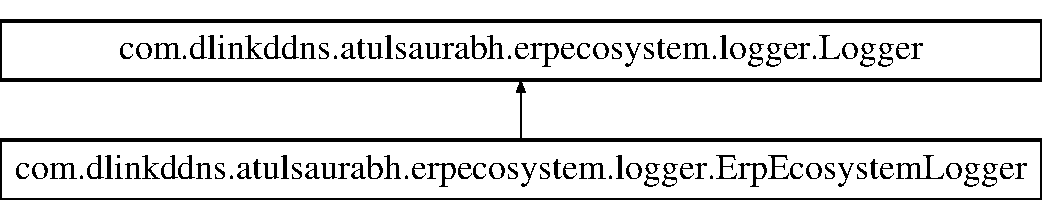
\includegraphics[height=2.000000cm]{interfacecom_1_1dlinkddns_1_1atulsaurabh_1_1erpecosystem_1_1logger_1_1_logger}
\end{center}
\end{figure}
\subsection*{Public Member Functions}
\begin{DoxyCompactItemize}
\item 
void \mbox{\hyperlink{interfacecom_1_1dlinkddns_1_1atulsaurabh_1_1erpecosystem_1_1logger_1_1_logger_ab1796d8ce066433e34409055fd5e7100}{log\+Fatal}} (String message)
\item 
void \mbox{\hyperlink{interfacecom_1_1dlinkddns_1_1atulsaurabh_1_1erpecosystem_1_1logger_1_1_logger_ae9763257a2db31ecdfd4675bcdcd3bd0}{log\+Fatal}} (Class error\+Class, String message)
\item 
void \mbox{\hyperlink{interfacecom_1_1dlinkddns_1_1atulsaurabh_1_1erpecosystem_1_1logger_1_1_logger_ad8e4ea32b41f7d225b8ea824af177a43}{log\+Fatal}} (Class error\+Class, String message, Throwable throwable)
\item 
void \mbox{\hyperlink{interfacecom_1_1dlinkddns_1_1atulsaurabh_1_1erpecosystem_1_1logger_1_1_logger_a45d119fc284eee3233ca247ec5f92e4c}{log\+All}} (String message)
\item 
void \mbox{\hyperlink{interfacecom_1_1dlinkddns_1_1atulsaurabh_1_1erpecosystem_1_1logger_1_1_logger_a232415e10e9da278b0bacf82309aef76}{log\+All}} (Class error\+Class, String message)
\item 
void \mbox{\hyperlink{interfacecom_1_1dlinkddns_1_1atulsaurabh_1_1erpecosystem_1_1logger_1_1_logger_aba1204d7d2383973ddf63e537e11086d}{log\+All}} (Class error\+Class, String message, Throwable throwable)
\item 
void \mbox{\hyperlink{interfacecom_1_1dlinkddns_1_1atulsaurabh_1_1erpecosystem_1_1logger_1_1_logger_af32bfcb68d536836f7bdb8618e4c1812}{set\+Rolling\+On}} (boolean rollingon)
\item 
boolean \mbox{\hyperlink{interfacecom_1_1dlinkddns_1_1atulsaurabh_1_1erpecosystem_1_1logger_1_1_logger_ae42fbcc81564437b6582b4c7ede3352b}{is\+Rolling\+On}} ()
\item 
void \mbox{\hyperlink{interfacecom_1_1dlinkddns_1_1atulsaurabh_1_1erpecosystem_1_1logger_1_1_logger_aceef18a85b09966b1ccf10c9927d0917}{set\+Date\+Pattern}} (String pattern)
\item 
String \mbox{\hyperlink{interfacecom_1_1dlinkddns_1_1atulsaurabh_1_1erpecosystem_1_1logger_1_1_logger_aab0359e92db242d1e64da4fc0b0fd638}{get\+Date\+Pattern}} ()
\item 
void \mbox{\hyperlink{interfacecom_1_1dlinkddns_1_1atulsaurabh_1_1erpecosystem_1_1logger_1_1_logger_add9a38d7fa3907aa924bdfe56f3fe5c3}{set\+Conversion\+Pattern}} (String pattern)
\item 
String \mbox{\hyperlink{interfacecom_1_1dlinkddns_1_1atulsaurabh_1_1erpecosystem_1_1logger_1_1_logger_ab9bd1ad5fb48fa4e46fb67fbbe2475f7}{get\+Conversion\+Pattern}} ()
\item 
void \mbox{\hyperlink{interfacecom_1_1dlinkddns_1_1atulsaurabh_1_1erpecosystem_1_1logger_1_1_logger_aab8d04f52fde89ff5e58d84b40e25144}{log\+Warning}} (String message)
\item 
void \mbox{\hyperlink{interfacecom_1_1dlinkddns_1_1atulsaurabh_1_1erpecosystem_1_1logger_1_1_logger_aa5df260afe6fcae92f5a9236b3b6a983}{log\+Warning}} (Class warning\+Class, String message)
\item 
void \mbox{\hyperlink{interfacecom_1_1dlinkddns_1_1atulsaurabh_1_1erpecosystem_1_1logger_1_1_logger_a05aa52bed792e7a4a3519dadaab2f4f3}{log\+Warning}} (Class warning\+Class, String message, Throwable throwable)
\item 
void \mbox{\hyperlink{interfacecom_1_1dlinkddns_1_1atulsaurabh_1_1erpecosystem_1_1logger_1_1_logger_a8671e0fd90d8f2fbb4024d7a73d9070d}{log\+Info}} (String message)
\item 
void \mbox{\hyperlink{interfacecom_1_1dlinkddns_1_1atulsaurabh_1_1erpecosystem_1_1logger_1_1_logger_a37e8723a5243a845e140d2edb6d7f701}{log\+Info}} (Class info\+Class, String message)
\item 
void \mbox{\hyperlink{interfacecom_1_1dlinkddns_1_1atulsaurabh_1_1erpecosystem_1_1logger_1_1_logger_a0a674a1745e0f50d11b1f8be2c4d1726}{log\+Info}} (Class info\+Class, String message, Throwable throwable)
\item 
void \mbox{\hyperlink{interfacecom_1_1dlinkddns_1_1atulsaurabh_1_1erpecosystem_1_1logger_1_1_logger_add9d87ff18f2b432002e2146b67b0f07}{log\+Debug}} (String message)
\item 
void \mbox{\hyperlink{interfacecom_1_1dlinkddns_1_1atulsaurabh_1_1erpecosystem_1_1logger_1_1_logger_a8e94c010b6e08d96550a8ddc4b2f408e}{log\+Debug}} (Class debug\+Class, String message)
\item 
void \mbox{\hyperlink{interfacecom_1_1dlinkddns_1_1atulsaurabh_1_1erpecosystem_1_1logger_1_1_logger_a95b44330997929adfe530e3c845e38f5}{log\+Debug}} (Class debug\+Class, String message, Throwable throwable)
\item 
void \mbox{\hyperlink{interfacecom_1_1dlinkddns_1_1atulsaurabh_1_1erpecosystem_1_1logger_1_1_logger_a0a9d496d0bbbd0afd87f13d38acb88e2}{log\+Error}} (String message)
\item 
void \mbox{\hyperlink{interfacecom_1_1dlinkddns_1_1atulsaurabh_1_1erpecosystem_1_1logger_1_1_logger_a1cf0d549875c44c1afd8cd01dc0af1d6}{log\+Error}} (Class error\+Class, String message)
\item 
void \mbox{\hyperlink{interfacecom_1_1dlinkddns_1_1atulsaurabh_1_1erpecosystem_1_1logger_1_1_logger_a0f7488f980f029dfa98c465877b3fbe6}{log\+Error}} (Class error\+Class, String message, Throwable throwable)
\end{DoxyCompactItemize}


\subsection{Detailed Description}
\begin{DoxyAuthor}{Author}
Atul Saurabh 
\end{DoxyAuthor}
\begin{DoxyVersion}{Version}
1.\+0 
\end{DoxyVersion}


Definition at line 13 of file Logger.\+java.



\subsection{Member Function Documentation}
\mbox{\Hypertarget{interfacecom_1_1dlinkddns_1_1atulsaurabh_1_1erpecosystem_1_1logger_1_1_logger_ab9bd1ad5fb48fa4e46fb67fbbe2475f7}\label{interfacecom_1_1dlinkddns_1_1atulsaurabh_1_1erpecosystem_1_1logger_1_1_logger_ab9bd1ad5fb48fa4e46fb67fbbe2475f7}} 
\index{com\+::dlinkddns\+::atulsaurabh\+::erpecosystem\+::logger\+::\+Logger@{com\+::dlinkddns\+::atulsaurabh\+::erpecosystem\+::logger\+::\+Logger}!get\+Conversion\+Pattern@{get\+Conversion\+Pattern}}
\index{get\+Conversion\+Pattern@{get\+Conversion\+Pattern}!com\+::dlinkddns\+::atulsaurabh\+::erpecosystem\+::logger\+::\+Logger@{com\+::dlinkddns\+::atulsaurabh\+::erpecosystem\+::logger\+::\+Logger}}
\subsubsection{\texorpdfstring{get\+Conversion\+Pattern()}{getConversionPattern()}}
{\footnotesize\ttfamily String com.\+dlinkddns.\+atulsaurabh.\+erpecosystem.\+logger.\+Logger.\+get\+Conversion\+Pattern (\begin{DoxyParamCaption}{ }\end{DoxyParamCaption})}

\begin{DoxyReturn}{Returns}
Format for printing message into log file 
\end{DoxyReturn}


Implemented in \mbox{\hyperlink{classcom_1_1dlinkddns_1_1atulsaurabh_1_1erpecosystem_1_1logger_1_1_erp_ecosystem_logger_a8f0373f6917c8fe5a3ddea2c2adf081c}{com.\+dlinkddns.\+atulsaurabh.\+erpecosystem.\+logger.\+Erp\+Ecosystem\+Logger}}.

\mbox{\Hypertarget{interfacecom_1_1dlinkddns_1_1atulsaurabh_1_1erpecosystem_1_1logger_1_1_logger_aab0359e92db242d1e64da4fc0b0fd638}\label{interfacecom_1_1dlinkddns_1_1atulsaurabh_1_1erpecosystem_1_1logger_1_1_logger_aab0359e92db242d1e64da4fc0b0fd638}} 
\index{com\+::dlinkddns\+::atulsaurabh\+::erpecosystem\+::logger\+::\+Logger@{com\+::dlinkddns\+::atulsaurabh\+::erpecosystem\+::logger\+::\+Logger}!get\+Date\+Pattern@{get\+Date\+Pattern}}
\index{get\+Date\+Pattern@{get\+Date\+Pattern}!com\+::dlinkddns\+::atulsaurabh\+::erpecosystem\+::logger\+::\+Logger@{com\+::dlinkddns\+::atulsaurabh\+::erpecosystem\+::logger\+::\+Logger}}
\subsubsection{\texorpdfstring{get\+Date\+Pattern()}{getDatePattern()}}
{\footnotesize\ttfamily String com.\+dlinkddns.\+atulsaurabh.\+erpecosystem.\+logger.\+Logger.\+get\+Date\+Pattern (\begin{DoxyParamCaption}{ }\end{DoxyParamCaption})}

\begin{DoxyReturn}{Returns}
date format used in log file 
\end{DoxyReturn}
\mbox{\Hypertarget{interfacecom_1_1dlinkddns_1_1atulsaurabh_1_1erpecosystem_1_1logger_1_1_logger_ae42fbcc81564437b6582b4c7ede3352b}\label{interfacecom_1_1dlinkddns_1_1atulsaurabh_1_1erpecosystem_1_1logger_1_1_logger_ae42fbcc81564437b6582b4c7ede3352b}} 
\index{com\+::dlinkddns\+::atulsaurabh\+::erpecosystem\+::logger\+::\+Logger@{com\+::dlinkddns\+::atulsaurabh\+::erpecosystem\+::logger\+::\+Logger}!is\+Rolling\+On@{is\+Rolling\+On}}
\index{is\+Rolling\+On@{is\+Rolling\+On}!com\+::dlinkddns\+::atulsaurabh\+::erpecosystem\+::logger\+::\+Logger@{com\+::dlinkddns\+::atulsaurabh\+::erpecosystem\+::logger\+::\+Logger}}
\subsubsection{\texorpdfstring{is\+Rolling\+On()}{isRollingOn()}}
{\footnotesize\ttfamily boolean com.\+dlinkddns.\+atulsaurabh.\+erpecosystem.\+logger.\+Logger.\+is\+Rolling\+On (\begin{DoxyParamCaption}{ }\end{DoxyParamCaption})}

\begin{DoxyReturn}{Returns}
the state of rolling 
\end{DoxyReturn}
\mbox{\Hypertarget{interfacecom_1_1dlinkddns_1_1atulsaurabh_1_1erpecosystem_1_1logger_1_1_logger_a45d119fc284eee3233ca247ec5f92e4c}\label{interfacecom_1_1dlinkddns_1_1atulsaurabh_1_1erpecosystem_1_1logger_1_1_logger_a45d119fc284eee3233ca247ec5f92e4c}} 
\index{com\+::dlinkddns\+::atulsaurabh\+::erpecosystem\+::logger\+::\+Logger@{com\+::dlinkddns\+::atulsaurabh\+::erpecosystem\+::logger\+::\+Logger}!log\+All@{log\+All}}
\index{log\+All@{log\+All}!com\+::dlinkddns\+::atulsaurabh\+::erpecosystem\+::logger\+::\+Logger@{com\+::dlinkddns\+::atulsaurabh\+::erpecosystem\+::logger\+::\+Logger}}
\subsubsection{\texorpdfstring{log\+All()}{logAll()}\hspace{0.1cm}{\footnotesize\ttfamily [1/3]}}
{\footnotesize\ttfamily void com.\+dlinkddns.\+atulsaurabh.\+erpecosystem.\+logger.\+Logger.\+log\+All (\begin{DoxyParamCaption}\item[{String}]{message }\end{DoxyParamCaption})}


\begin{DoxyParams}{Parameters}
{\em message} & Any message to be logged in \\
\hline
\end{DoxyParams}


Implemented in \mbox{\hyperlink{classcom_1_1dlinkddns_1_1atulsaurabh_1_1erpecosystem_1_1logger_1_1_erp_ecosystem_logger_a360f98d9c9cf93c49fbb0a6a1e3e922f}{com.\+dlinkddns.\+atulsaurabh.\+erpecosystem.\+logger.\+Erp\+Ecosystem\+Logger}}.

\mbox{\Hypertarget{interfacecom_1_1dlinkddns_1_1atulsaurabh_1_1erpecosystem_1_1logger_1_1_logger_a232415e10e9da278b0bacf82309aef76}\label{interfacecom_1_1dlinkddns_1_1atulsaurabh_1_1erpecosystem_1_1logger_1_1_logger_a232415e10e9da278b0bacf82309aef76}} 
\index{com\+::dlinkddns\+::atulsaurabh\+::erpecosystem\+::logger\+::\+Logger@{com\+::dlinkddns\+::atulsaurabh\+::erpecosystem\+::logger\+::\+Logger}!log\+All@{log\+All}}
\index{log\+All@{log\+All}!com\+::dlinkddns\+::atulsaurabh\+::erpecosystem\+::logger\+::\+Logger@{com\+::dlinkddns\+::atulsaurabh\+::erpecosystem\+::logger\+::\+Logger}}
\subsubsection{\texorpdfstring{log\+All()}{logAll()}\hspace{0.1cm}{\footnotesize\ttfamily [2/3]}}
{\footnotesize\ttfamily void com.\+dlinkddns.\+atulsaurabh.\+erpecosystem.\+logger.\+Logger.\+log\+All (\begin{DoxyParamCaption}\item[{Class}]{error\+Class,  }\item[{String}]{message }\end{DoxyParamCaption})}


\begin{DoxyParams}{Parameters}
{\em error\+Class} & Any error or warning or info etc generating class \\
\hline
{\em message} & Any message to be logged in \\
\hline
\end{DoxyParams}


Implemented in \mbox{\hyperlink{classcom_1_1dlinkddns_1_1atulsaurabh_1_1erpecosystem_1_1logger_1_1_erp_ecosystem_logger_a5bea48485386781a9eee8a78c2e2c9be}{com.\+dlinkddns.\+atulsaurabh.\+erpecosystem.\+logger.\+Erp\+Ecosystem\+Logger}}.

\mbox{\Hypertarget{interfacecom_1_1dlinkddns_1_1atulsaurabh_1_1erpecosystem_1_1logger_1_1_logger_aba1204d7d2383973ddf63e537e11086d}\label{interfacecom_1_1dlinkddns_1_1atulsaurabh_1_1erpecosystem_1_1logger_1_1_logger_aba1204d7d2383973ddf63e537e11086d}} 
\index{com\+::dlinkddns\+::atulsaurabh\+::erpecosystem\+::logger\+::\+Logger@{com\+::dlinkddns\+::atulsaurabh\+::erpecosystem\+::logger\+::\+Logger}!log\+All@{log\+All}}
\index{log\+All@{log\+All}!com\+::dlinkddns\+::atulsaurabh\+::erpecosystem\+::logger\+::\+Logger@{com\+::dlinkddns\+::atulsaurabh\+::erpecosystem\+::logger\+::\+Logger}}
\subsubsection{\texorpdfstring{log\+All()}{logAll()}\hspace{0.1cm}{\footnotesize\ttfamily [3/3]}}
{\footnotesize\ttfamily void com.\+dlinkddns.\+atulsaurabh.\+erpecosystem.\+logger.\+Logger.\+log\+All (\begin{DoxyParamCaption}\item[{Class}]{error\+Class,  }\item[{String}]{message,  }\item[{Throwable}]{throwable }\end{DoxyParamCaption})}


\begin{DoxyParams}{Parameters}
{\em error\+Class} & Any error or warning or info etc generating class \\
\hline
{\em message} & Any message to be logged in \\
\hline
{\em throwable} & Any object representing warning,error,fatal etc. \\
\hline
\end{DoxyParams}


Implemented in \mbox{\hyperlink{classcom_1_1dlinkddns_1_1atulsaurabh_1_1erpecosystem_1_1logger_1_1_erp_ecosystem_logger_a2706d4afe3cf3f8dad301d43851181ce}{com.\+dlinkddns.\+atulsaurabh.\+erpecosystem.\+logger.\+Erp\+Ecosystem\+Logger}}.

\mbox{\Hypertarget{interfacecom_1_1dlinkddns_1_1atulsaurabh_1_1erpecosystem_1_1logger_1_1_logger_add9d87ff18f2b432002e2146b67b0f07}\label{interfacecom_1_1dlinkddns_1_1atulsaurabh_1_1erpecosystem_1_1logger_1_1_logger_add9d87ff18f2b432002e2146b67b0f07}} 
\index{com\+::dlinkddns\+::atulsaurabh\+::erpecosystem\+::logger\+::\+Logger@{com\+::dlinkddns\+::atulsaurabh\+::erpecosystem\+::logger\+::\+Logger}!log\+Debug@{log\+Debug}}
\index{log\+Debug@{log\+Debug}!com\+::dlinkddns\+::atulsaurabh\+::erpecosystem\+::logger\+::\+Logger@{com\+::dlinkddns\+::atulsaurabh\+::erpecosystem\+::logger\+::\+Logger}}
\subsubsection{\texorpdfstring{log\+Debug()}{logDebug()}\hspace{0.1cm}{\footnotesize\ttfamily [1/3]}}
{\footnotesize\ttfamily void com.\+dlinkddns.\+atulsaurabh.\+erpecosystem.\+logger.\+Logger.\+log\+Debug (\begin{DoxyParamCaption}\item[{String}]{message }\end{DoxyParamCaption})}



Implemented in \mbox{\hyperlink{classcom_1_1dlinkddns_1_1atulsaurabh_1_1erpecosystem_1_1logger_1_1_erp_ecosystem_logger_a220bd030f8fe67c986972c3925727196}{com.\+dlinkddns.\+atulsaurabh.\+erpecosystem.\+logger.\+Erp\+Ecosystem\+Logger}}.

\mbox{\Hypertarget{interfacecom_1_1dlinkddns_1_1atulsaurabh_1_1erpecosystem_1_1logger_1_1_logger_a8e94c010b6e08d96550a8ddc4b2f408e}\label{interfacecom_1_1dlinkddns_1_1atulsaurabh_1_1erpecosystem_1_1logger_1_1_logger_a8e94c010b6e08d96550a8ddc4b2f408e}} 
\index{com\+::dlinkddns\+::atulsaurabh\+::erpecosystem\+::logger\+::\+Logger@{com\+::dlinkddns\+::atulsaurabh\+::erpecosystem\+::logger\+::\+Logger}!log\+Debug@{log\+Debug}}
\index{log\+Debug@{log\+Debug}!com\+::dlinkddns\+::atulsaurabh\+::erpecosystem\+::logger\+::\+Logger@{com\+::dlinkddns\+::atulsaurabh\+::erpecosystem\+::logger\+::\+Logger}}
\subsubsection{\texorpdfstring{log\+Debug()}{logDebug()}\hspace{0.1cm}{\footnotesize\ttfamily [2/3]}}
{\footnotesize\ttfamily void com.\+dlinkddns.\+atulsaurabh.\+erpecosystem.\+logger.\+Logger.\+log\+Debug (\begin{DoxyParamCaption}\item[{Class}]{debug\+Class,  }\item[{String}]{message }\end{DoxyParamCaption})}



Implemented in \mbox{\hyperlink{classcom_1_1dlinkddns_1_1atulsaurabh_1_1erpecosystem_1_1logger_1_1_erp_ecosystem_logger_a80d54c08b8d233dc1782e1f85bdde19a}{com.\+dlinkddns.\+atulsaurabh.\+erpecosystem.\+logger.\+Erp\+Ecosystem\+Logger}}.

\mbox{\Hypertarget{interfacecom_1_1dlinkddns_1_1atulsaurabh_1_1erpecosystem_1_1logger_1_1_logger_a95b44330997929adfe530e3c845e38f5}\label{interfacecom_1_1dlinkddns_1_1atulsaurabh_1_1erpecosystem_1_1logger_1_1_logger_a95b44330997929adfe530e3c845e38f5}} 
\index{com\+::dlinkddns\+::atulsaurabh\+::erpecosystem\+::logger\+::\+Logger@{com\+::dlinkddns\+::atulsaurabh\+::erpecosystem\+::logger\+::\+Logger}!log\+Debug@{log\+Debug}}
\index{log\+Debug@{log\+Debug}!com\+::dlinkddns\+::atulsaurabh\+::erpecosystem\+::logger\+::\+Logger@{com\+::dlinkddns\+::atulsaurabh\+::erpecosystem\+::logger\+::\+Logger}}
\subsubsection{\texorpdfstring{log\+Debug()}{logDebug()}\hspace{0.1cm}{\footnotesize\ttfamily [3/3]}}
{\footnotesize\ttfamily void com.\+dlinkddns.\+atulsaurabh.\+erpecosystem.\+logger.\+Logger.\+log\+Debug (\begin{DoxyParamCaption}\item[{Class}]{debug\+Class,  }\item[{String}]{message,  }\item[{Throwable}]{throwable }\end{DoxyParamCaption})}



Implemented in \mbox{\hyperlink{classcom_1_1dlinkddns_1_1atulsaurabh_1_1erpecosystem_1_1logger_1_1_erp_ecosystem_logger_a40e19afc6e72a31339e4eec00132c166}{com.\+dlinkddns.\+atulsaurabh.\+erpecosystem.\+logger.\+Erp\+Ecosystem\+Logger}}.

\mbox{\Hypertarget{interfacecom_1_1dlinkddns_1_1atulsaurabh_1_1erpecosystem_1_1logger_1_1_logger_a0a9d496d0bbbd0afd87f13d38acb88e2}\label{interfacecom_1_1dlinkddns_1_1atulsaurabh_1_1erpecosystem_1_1logger_1_1_logger_a0a9d496d0bbbd0afd87f13d38acb88e2}} 
\index{com\+::dlinkddns\+::atulsaurabh\+::erpecosystem\+::logger\+::\+Logger@{com\+::dlinkddns\+::atulsaurabh\+::erpecosystem\+::logger\+::\+Logger}!log\+Error@{log\+Error}}
\index{log\+Error@{log\+Error}!com\+::dlinkddns\+::atulsaurabh\+::erpecosystem\+::logger\+::\+Logger@{com\+::dlinkddns\+::atulsaurabh\+::erpecosystem\+::logger\+::\+Logger}}
\subsubsection{\texorpdfstring{log\+Error()}{logError()}\hspace{0.1cm}{\footnotesize\ttfamily [1/3]}}
{\footnotesize\ttfamily void com.\+dlinkddns.\+atulsaurabh.\+erpecosystem.\+logger.\+Logger.\+log\+Error (\begin{DoxyParamCaption}\item[{String}]{message }\end{DoxyParamCaption})}



Implemented in \mbox{\hyperlink{classcom_1_1dlinkddns_1_1atulsaurabh_1_1erpecosystem_1_1logger_1_1_erp_ecosystem_logger_ab9553bd3b9e717accdc9c2d0ee13371e}{com.\+dlinkddns.\+atulsaurabh.\+erpecosystem.\+logger.\+Erp\+Ecosystem\+Logger}}.

\mbox{\Hypertarget{interfacecom_1_1dlinkddns_1_1atulsaurabh_1_1erpecosystem_1_1logger_1_1_logger_a1cf0d549875c44c1afd8cd01dc0af1d6}\label{interfacecom_1_1dlinkddns_1_1atulsaurabh_1_1erpecosystem_1_1logger_1_1_logger_a1cf0d549875c44c1afd8cd01dc0af1d6}} 
\index{com\+::dlinkddns\+::atulsaurabh\+::erpecosystem\+::logger\+::\+Logger@{com\+::dlinkddns\+::atulsaurabh\+::erpecosystem\+::logger\+::\+Logger}!log\+Error@{log\+Error}}
\index{log\+Error@{log\+Error}!com\+::dlinkddns\+::atulsaurabh\+::erpecosystem\+::logger\+::\+Logger@{com\+::dlinkddns\+::atulsaurabh\+::erpecosystem\+::logger\+::\+Logger}}
\subsubsection{\texorpdfstring{log\+Error()}{logError()}\hspace{0.1cm}{\footnotesize\ttfamily [2/3]}}
{\footnotesize\ttfamily void com.\+dlinkddns.\+atulsaurabh.\+erpecosystem.\+logger.\+Logger.\+log\+Error (\begin{DoxyParamCaption}\item[{Class}]{error\+Class,  }\item[{String}]{message }\end{DoxyParamCaption})}



Implemented in \mbox{\hyperlink{classcom_1_1dlinkddns_1_1atulsaurabh_1_1erpecosystem_1_1logger_1_1_erp_ecosystem_logger_aa561000b385ff39f9d8171a91e831c2d}{com.\+dlinkddns.\+atulsaurabh.\+erpecosystem.\+logger.\+Erp\+Ecosystem\+Logger}}.

\mbox{\Hypertarget{interfacecom_1_1dlinkddns_1_1atulsaurabh_1_1erpecosystem_1_1logger_1_1_logger_a0f7488f980f029dfa98c465877b3fbe6}\label{interfacecom_1_1dlinkddns_1_1atulsaurabh_1_1erpecosystem_1_1logger_1_1_logger_a0f7488f980f029dfa98c465877b3fbe6}} 
\index{com\+::dlinkddns\+::atulsaurabh\+::erpecosystem\+::logger\+::\+Logger@{com\+::dlinkddns\+::atulsaurabh\+::erpecosystem\+::logger\+::\+Logger}!log\+Error@{log\+Error}}
\index{log\+Error@{log\+Error}!com\+::dlinkddns\+::atulsaurabh\+::erpecosystem\+::logger\+::\+Logger@{com\+::dlinkddns\+::atulsaurabh\+::erpecosystem\+::logger\+::\+Logger}}
\subsubsection{\texorpdfstring{log\+Error()}{logError()}\hspace{0.1cm}{\footnotesize\ttfamily [3/3]}}
{\footnotesize\ttfamily void com.\+dlinkddns.\+atulsaurabh.\+erpecosystem.\+logger.\+Logger.\+log\+Error (\begin{DoxyParamCaption}\item[{Class}]{error\+Class,  }\item[{String}]{message,  }\item[{Throwable}]{throwable }\end{DoxyParamCaption})}



Implemented in \mbox{\hyperlink{classcom_1_1dlinkddns_1_1atulsaurabh_1_1erpecosystem_1_1logger_1_1_erp_ecosystem_logger_a25316b3eabb66eaecba45d638c420b2b}{com.\+dlinkddns.\+atulsaurabh.\+erpecosystem.\+logger.\+Erp\+Ecosystem\+Logger}}.

\mbox{\Hypertarget{interfacecom_1_1dlinkddns_1_1atulsaurabh_1_1erpecosystem_1_1logger_1_1_logger_ab1796d8ce066433e34409055fd5e7100}\label{interfacecom_1_1dlinkddns_1_1atulsaurabh_1_1erpecosystem_1_1logger_1_1_logger_ab1796d8ce066433e34409055fd5e7100}} 
\index{com\+::dlinkddns\+::atulsaurabh\+::erpecosystem\+::logger\+::\+Logger@{com\+::dlinkddns\+::atulsaurabh\+::erpecosystem\+::logger\+::\+Logger}!log\+Fatal@{log\+Fatal}}
\index{log\+Fatal@{log\+Fatal}!com\+::dlinkddns\+::atulsaurabh\+::erpecosystem\+::logger\+::\+Logger@{com\+::dlinkddns\+::atulsaurabh\+::erpecosystem\+::logger\+::\+Logger}}
\subsubsection{\texorpdfstring{log\+Fatal()}{logFatal()}\hspace{0.1cm}{\footnotesize\ttfamily [1/3]}}
{\footnotesize\ttfamily void com.\+dlinkddns.\+atulsaurabh.\+erpecosystem.\+logger.\+Logger.\+log\+Fatal (\begin{DoxyParamCaption}\item[{String}]{message }\end{DoxyParamCaption})}


\begin{DoxyParams}{Parameters}
{\em message} & Fatal message to be logged \\
\hline
\end{DoxyParams}


Implemented in \mbox{\hyperlink{classcom_1_1dlinkddns_1_1atulsaurabh_1_1erpecosystem_1_1logger_1_1_erp_ecosystem_logger_a366c4448e35274f7b1edec8112fb2553}{com.\+dlinkddns.\+atulsaurabh.\+erpecosystem.\+logger.\+Erp\+Ecosystem\+Logger}}.

\mbox{\Hypertarget{interfacecom_1_1dlinkddns_1_1atulsaurabh_1_1erpecosystem_1_1logger_1_1_logger_ae9763257a2db31ecdfd4675bcdcd3bd0}\label{interfacecom_1_1dlinkddns_1_1atulsaurabh_1_1erpecosystem_1_1logger_1_1_logger_ae9763257a2db31ecdfd4675bcdcd3bd0}} 
\index{com\+::dlinkddns\+::atulsaurabh\+::erpecosystem\+::logger\+::\+Logger@{com\+::dlinkddns\+::atulsaurabh\+::erpecosystem\+::logger\+::\+Logger}!log\+Fatal@{log\+Fatal}}
\index{log\+Fatal@{log\+Fatal}!com\+::dlinkddns\+::atulsaurabh\+::erpecosystem\+::logger\+::\+Logger@{com\+::dlinkddns\+::atulsaurabh\+::erpecosystem\+::logger\+::\+Logger}}
\subsubsection{\texorpdfstring{log\+Fatal()}{logFatal()}\hspace{0.1cm}{\footnotesize\ttfamily [2/3]}}
{\footnotesize\ttfamily void com.\+dlinkddns.\+atulsaurabh.\+erpecosystem.\+logger.\+Logger.\+log\+Fatal (\begin{DoxyParamCaption}\item[{Class}]{error\+Class,  }\item[{String}]{message }\end{DoxyParamCaption})}


\begin{DoxyParams}{Parameters}
{\em error\+Class} & Class where exception is caught \\
\hline
{\em message} & Fatal message to be logged \\
\hline
\end{DoxyParams}


Implemented in \mbox{\hyperlink{classcom_1_1dlinkddns_1_1atulsaurabh_1_1erpecosystem_1_1logger_1_1_erp_ecosystem_logger_ae9010d95c151f9940d3c4bcbb9a2f4b1}{com.\+dlinkddns.\+atulsaurabh.\+erpecosystem.\+logger.\+Erp\+Ecosystem\+Logger}}.

\mbox{\Hypertarget{interfacecom_1_1dlinkddns_1_1atulsaurabh_1_1erpecosystem_1_1logger_1_1_logger_ad8e4ea32b41f7d225b8ea824af177a43}\label{interfacecom_1_1dlinkddns_1_1atulsaurabh_1_1erpecosystem_1_1logger_1_1_logger_ad8e4ea32b41f7d225b8ea824af177a43}} 
\index{com\+::dlinkddns\+::atulsaurabh\+::erpecosystem\+::logger\+::\+Logger@{com\+::dlinkddns\+::atulsaurabh\+::erpecosystem\+::logger\+::\+Logger}!log\+Fatal@{log\+Fatal}}
\index{log\+Fatal@{log\+Fatal}!com\+::dlinkddns\+::atulsaurabh\+::erpecosystem\+::logger\+::\+Logger@{com\+::dlinkddns\+::atulsaurabh\+::erpecosystem\+::logger\+::\+Logger}}
\subsubsection{\texorpdfstring{log\+Fatal()}{logFatal()}\hspace{0.1cm}{\footnotesize\ttfamily [3/3]}}
{\footnotesize\ttfamily void com.\+dlinkddns.\+atulsaurabh.\+erpecosystem.\+logger.\+Logger.\+log\+Fatal (\begin{DoxyParamCaption}\item[{Class}]{error\+Class,  }\item[{String}]{message,  }\item[{Throwable}]{throwable }\end{DoxyParamCaption})}


\begin{DoxyParams}{Parameters}
{\em error\+Class} & Class where exception is caught \\
\hline
{\em message} & Fatal message to be logged \\
\hline
{\em throwable} & The instance of exception generated from stack trace \\
\hline
\end{DoxyParams}


Implemented in \mbox{\hyperlink{classcom_1_1dlinkddns_1_1atulsaurabh_1_1erpecosystem_1_1logger_1_1_erp_ecosystem_logger_a3def664f09892d36bbff6343fa8f3d6f}{com.\+dlinkddns.\+atulsaurabh.\+erpecosystem.\+logger.\+Erp\+Ecosystem\+Logger}}.

\mbox{\Hypertarget{interfacecom_1_1dlinkddns_1_1atulsaurabh_1_1erpecosystem_1_1logger_1_1_logger_a8671e0fd90d8f2fbb4024d7a73d9070d}\label{interfacecom_1_1dlinkddns_1_1atulsaurabh_1_1erpecosystem_1_1logger_1_1_logger_a8671e0fd90d8f2fbb4024d7a73d9070d}} 
\index{com\+::dlinkddns\+::atulsaurabh\+::erpecosystem\+::logger\+::\+Logger@{com\+::dlinkddns\+::atulsaurabh\+::erpecosystem\+::logger\+::\+Logger}!log\+Info@{log\+Info}}
\index{log\+Info@{log\+Info}!com\+::dlinkddns\+::atulsaurabh\+::erpecosystem\+::logger\+::\+Logger@{com\+::dlinkddns\+::atulsaurabh\+::erpecosystem\+::logger\+::\+Logger}}
\subsubsection{\texorpdfstring{log\+Info()}{logInfo()}\hspace{0.1cm}{\footnotesize\ttfamily [1/3]}}
{\footnotesize\ttfamily void com.\+dlinkddns.\+atulsaurabh.\+erpecosystem.\+logger.\+Logger.\+log\+Info (\begin{DoxyParamCaption}\item[{String}]{message }\end{DoxyParamCaption})}



Implemented in \mbox{\hyperlink{classcom_1_1dlinkddns_1_1atulsaurabh_1_1erpecosystem_1_1logger_1_1_erp_ecosystem_logger_a25071d05590b133a88f8b2f35092ebd7}{com.\+dlinkddns.\+atulsaurabh.\+erpecosystem.\+logger.\+Erp\+Ecosystem\+Logger}}.

\mbox{\Hypertarget{interfacecom_1_1dlinkddns_1_1atulsaurabh_1_1erpecosystem_1_1logger_1_1_logger_a37e8723a5243a845e140d2edb6d7f701}\label{interfacecom_1_1dlinkddns_1_1atulsaurabh_1_1erpecosystem_1_1logger_1_1_logger_a37e8723a5243a845e140d2edb6d7f701}} 
\index{com\+::dlinkddns\+::atulsaurabh\+::erpecosystem\+::logger\+::\+Logger@{com\+::dlinkddns\+::atulsaurabh\+::erpecosystem\+::logger\+::\+Logger}!log\+Info@{log\+Info}}
\index{log\+Info@{log\+Info}!com\+::dlinkddns\+::atulsaurabh\+::erpecosystem\+::logger\+::\+Logger@{com\+::dlinkddns\+::atulsaurabh\+::erpecosystem\+::logger\+::\+Logger}}
\subsubsection{\texorpdfstring{log\+Info()}{logInfo()}\hspace{0.1cm}{\footnotesize\ttfamily [2/3]}}
{\footnotesize\ttfamily void com.\+dlinkddns.\+atulsaurabh.\+erpecosystem.\+logger.\+Logger.\+log\+Info (\begin{DoxyParamCaption}\item[{Class}]{info\+Class,  }\item[{String}]{message }\end{DoxyParamCaption})}



Implemented in \mbox{\hyperlink{classcom_1_1dlinkddns_1_1atulsaurabh_1_1erpecosystem_1_1logger_1_1_erp_ecosystem_logger_a70838215b194b2f9771cec61a7f660c0}{com.\+dlinkddns.\+atulsaurabh.\+erpecosystem.\+logger.\+Erp\+Ecosystem\+Logger}}.

\mbox{\Hypertarget{interfacecom_1_1dlinkddns_1_1atulsaurabh_1_1erpecosystem_1_1logger_1_1_logger_a0a674a1745e0f50d11b1f8be2c4d1726}\label{interfacecom_1_1dlinkddns_1_1atulsaurabh_1_1erpecosystem_1_1logger_1_1_logger_a0a674a1745e0f50d11b1f8be2c4d1726}} 
\index{com\+::dlinkddns\+::atulsaurabh\+::erpecosystem\+::logger\+::\+Logger@{com\+::dlinkddns\+::atulsaurabh\+::erpecosystem\+::logger\+::\+Logger}!log\+Info@{log\+Info}}
\index{log\+Info@{log\+Info}!com\+::dlinkddns\+::atulsaurabh\+::erpecosystem\+::logger\+::\+Logger@{com\+::dlinkddns\+::atulsaurabh\+::erpecosystem\+::logger\+::\+Logger}}
\subsubsection{\texorpdfstring{log\+Info()}{logInfo()}\hspace{0.1cm}{\footnotesize\ttfamily [3/3]}}
{\footnotesize\ttfamily void com.\+dlinkddns.\+atulsaurabh.\+erpecosystem.\+logger.\+Logger.\+log\+Info (\begin{DoxyParamCaption}\item[{Class}]{info\+Class,  }\item[{String}]{message,  }\item[{Throwable}]{throwable }\end{DoxyParamCaption})}



Implemented in \mbox{\hyperlink{classcom_1_1dlinkddns_1_1atulsaurabh_1_1erpecosystem_1_1logger_1_1_erp_ecosystem_logger_ad6718b3031cb8032127659aeac49d803}{com.\+dlinkddns.\+atulsaurabh.\+erpecosystem.\+logger.\+Erp\+Ecosystem\+Logger}}.

\mbox{\Hypertarget{interfacecom_1_1dlinkddns_1_1atulsaurabh_1_1erpecosystem_1_1logger_1_1_logger_aab8d04f52fde89ff5e58d84b40e25144}\label{interfacecom_1_1dlinkddns_1_1atulsaurabh_1_1erpecosystem_1_1logger_1_1_logger_aab8d04f52fde89ff5e58d84b40e25144}} 
\index{com\+::dlinkddns\+::atulsaurabh\+::erpecosystem\+::logger\+::\+Logger@{com\+::dlinkddns\+::atulsaurabh\+::erpecosystem\+::logger\+::\+Logger}!log\+Warning@{log\+Warning}}
\index{log\+Warning@{log\+Warning}!com\+::dlinkddns\+::atulsaurabh\+::erpecosystem\+::logger\+::\+Logger@{com\+::dlinkddns\+::atulsaurabh\+::erpecosystem\+::logger\+::\+Logger}}
\subsubsection{\texorpdfstring{log\+Warning()}{logWarning()}\hspace{0.1cm}{\footnotesize\ttfamily [1/3]}}
{\footnotesize\ttfamily void com.\+dlinkddns.\+atulsaurabh.\+erpecosystem.\+logger.\+Logger.\+log\+Warning (\begin{DoxyParamCaption}\item[{String}]{message }\end{DoxyParamCaption})}



Implemented in \mbox{\hyperlink{classcom_1_1dlinkddns_1_1atulsaurabh_1_1erpecosystem_1_1logger_1_1_erp_ecosystem_logger_a4a4c244511da1da97773a5a7933552d2}{com.\+dlinkddns.\+atulsaurabh.\+erpecosystem.\+logger.\+Erp\+Ecosystem\+Logger}}.

\mbox{\Hypertarget{interfacecom_1_1dlinkddns_1_1atulsaurabh_1_1erpecosystem_1_1logger_1_1_logger_aa5df260afe6fcae92f5a9236b3b6a983}\label{interfacecom_1_1dlinkddns_1_1atulsaurabh_1_1erpecosystem_1_1logger_1_1_logger_aa5df260afe6fcae92f5a9236b3b6a983}} 
\index{com\+::dlinkddns\+::atulsaurabh\+::erpecosystem\+::logger\+::\+Logger@{com\+::dlinkddns\+::atulsaurabh\+::erpecosystem\+::logger\+::\+Logger}!log\+Warning@{log\+Warning}}
\index{log\+Warning@{log\+Warning}!com\+::dlinkddns\+::atulsaurabh\+::erpecosystem\+::logger\+::\+Logger@{com\+::dlinkddns\+::atulsaurabh\+::erpecosystem\+::logger\+::\+Logger}}
\subsubsection{\texorpdfstring{log\+Warning()}{logWarning()}\hspace{0.1cm}{\footnotesize\ttfamily [2/3]}}
{\footnotesize\ttfamily void com.\+dlinkddns.\+atulsaurabh.\+erpecosystem.\+logger.\+Logger.\+log\+Warning (\begin{DoxyParamCaption}\item[{Class}]{warning\+Class,  }\item[{String}]{message }\end{DoxyParamCaption})}



Implemented in \mbox{\hyperlink{classcom_1_1dlinkddns_1_1atulsaurabh_1_1erpecosystem_1_1logger_1_1_erp_ecosystem_logger_a7f8550d69fe0f6062f80c0cda4c74d87}{com.\+dlinkddns.\+atulsaurabh.\+erpecosystem.\+logger.\+Erp\+Ecosystem\+Logger}}.

\mbox{\Hypertarget{interfacecom_1_1dlinkddns_1_1atulsaurabh_1_1erpecosystem_1_1logger_1_1_logger_a05aa52bed792e7a4a3519dadaab2f4f3}\label{interfacecom_1_1dlinkddns_1_1atulsaurabh_1_1erpecosystem_1_1logger_1_1_logger_a05aa52bed792e7a4a3519dadaab2f4f3}} 
\index{com\+::dlinkddns\+::atulsaurabh\+::erpecosystem\+::logger\+::\+Logger@{com\+::dlinkddns\+::atulsaurabh\+::erpecosystem\+::logger\+::\+Logger}!log\+Warning@{log\+Warning}}
\index{log\+Warning@{log\+Warning}!com\+::dlinkddns\+::atulsaurabh\+::erpecosystem\+::logger\+::\+Logger@{com\+::dlinkddns\+::atulsaurabh\+::erpecosystem\+::logger\+::\+Logger}}
\subsubsection{\texorpdfstring{log\+Warning()}{logWarning()}\hspace{0.1cm}{\footnotesize\ttfamily [3/3]}}
{\footnotesize\ttfamily void com.\+dlinkddns.\+atulsaurabh.\+erpecosystem.\+logger.\+Logger.\+log\+Warning (\begin{DoxyParamCaption}\item[{Class}]{warning\+Class,  }\item[{String}]{message,  }\item[{Throwable}]{throwable }\end{DoxyParamCaption})}



Implemented in \mbox{\hyperlink{classcom_1_1dlinkddns_1_1atulsaurabh_1_1erpecosystem_1_1logger_1_1_erp_ecosystem_logger_a432114edc56c223b7b5764348641ea24}{com.\+dlinkddns.\+atulsaurabh.\+erpecosystem.\+logger.\+Erp\+Ecosystem\+Logger}}.

\mbox{\Hypertarget{interfacecom_1_1dlinkddns_1_1atulsaurabh_1_1erpecosystem_1_1logger_1_1_logger_add9a38d7fa3907aa924bdfe56f3fe5c3}\label{interfacecom_1_1dlinkddns_1_1atulsaurabh_1_1erpecosystem_1_1logger_1_1_logger_add9a38d7fa3907aa924bdfe56f3fe5c3}} 
\index{com\+::dlinkddns\+::atulsaurabh\+::erpecosystem\+::logger\+::\+Logger@{com\+::dlinkddns\+::atulsaurabh\+::erpecosystem\+::logger\+::\+Logger}!set\+Conversion\+Pattern@{set\+Conversion\+Pattern}}
\index{set\+Conversion\+Pattern@{set\+Conversion\+Pattern}!com\+::dlinkddns\+::atulsaurabh\+::erpecosystem\+::logger\+::\+Logger@{com\+::dlinkddns\+::atulsaurabh\+::erpecosystem\+::logger\+::\+Logger}}
\subsubsection{\texorpdfstring{set\+Conversion\+Pattern()}{setConversionPattern()}}
{\footnotesize\ttfamily void com.\+dlinkddns.\+atulsaurabh.\+erpecosystem.\+logger.\+Logger.\+set\+Conversion\+Pattern (\begin{DoxyParamCaption}\item[{String}]{pattern }\end{DoxyParamCaption})}


\begin{DoxyParams}{Parameters}
{\em pattern} & Format for printing message into log file \\
\hline
\end{DoxyParams}


Implemented in \mbox{\hyperlink{classcom_1_1dlinkddns_1_1atulsaurabh_1_1erpecosystem_1_1logger_1_1_erp_ecosystem_logger_a16d43ce13e22b9fae1b9e3b55a086b06}{com.\+dlinkddns.\+atulsaurabh.\+erpecosystem.\+logger.\+Erp\+Ecosystem\+Logger}}.

\mbox{\Hypertarget{interfacecom_1_1dlinkddns_1_1atulsaurabh_1_1erpecosystem_1_1logger_1_1_logger_aceef18a85b09966b1ccf10c9927d0917}\label{interfacecom_1_1dlinkddns_1_1atulsaurabh_1_1erpecosystem_1_1logger_1_1_logger_aceef18a85b09966b1ccf10c9927d0917}} 
\index{com\+::dlinkddns\+::atulsaurabh\+::erpecosystem\+::logger\+::\+Logger@{com\+::dlinkddns\+::atulsaurabh\+::erpecosystem\+::logger\+::\+Logger}!set\+Date\+Pattern@{set\+Date\+Pattern}}
\index{set\+Date\+Pattern@{set\+Date\+Pattern}!com\+::dlinkddns\+::atulsaurabh\+::erpecosystem\+::logger\+::\+Logger@{com\+::dlinkddns\+::atulsaurabh\+::erpecosystem\+::logger\+::\+Logger}}
\subsubsection{\texorpdfstring{set\+Date\+Pattern()}{setDatePattern()}}
{\footnotesize\ttfamily void com.\+dlinkddns.\+atulsaurabh.\+erpecosystem.\+logger.\+Logger.\+set\+Date\+Pattern (\begin{DoxyParamCaption}\item[{String}]{pattern }\end{DoxyParamCaption})}


\begin{DoxyParams}{Parameters}
{\em pattern} & The pattern for date used in log file \\
\hline
\end{DoxyParams}
\mbox{\Hypertarget{interfacecom_1_1dlinkddns_1_1atulsaurabh_1_1erpecosystem_1_1logger_1_1_logger_af32bfcb68d536836f7bdb8618e4c1812}\label{interfacecom_1_1dlinkddns_1_1atulsaurabh_1_1erpecosystem_1_1logger_1_1_logger_af32bfcb68d536836f7bdb8618e4c1812}} 
\index{com\+::dlinkddns\+::atulsaurabh\+::erpecosystem\+::logger\+::\+Logger@{com\+::dlinkddns\+::atulsaurabh\+::erpecosystem\+::logger\+::\+Logger}!set\+Rolling\+On@{set\+Rolling\+On}}
\index{set\+Rolling\+On@{set\+Rolling\+On}!com\+::dlinkddns\+::atulsaurabh\+::erpecosystem\+::logger\+::\+Logger@{com\+::dlinkddns\+::atulsaurabh\+::erpecosystem\+::logger\+::\+Logger}}
\subsubsection{\texorpdfstring{set\+Rolling\+On()}{setRollingOn()}}
{\footnotesize\ttfamily void com.\+dlinkddns.\+atulsaurabh.\+erpecosystem.\+logger.\+Logger.\+set\+Rolling\+On (\begin{DoxyParamCaption}\item[{boolean}]{rollingon }\end{DoxyParamCaption})}


\begin{DoxyParams}{Parameters}
{\em rollingon} & make rolling on so that log can be generated and stored date wise \\
\hline
\end{DoxyParams}


The documentation for this interface was generated from the following file\+:\begin{DoxyCompactItemize}
\item 
C\+:/myworkplace/projects/erpecosystem/src/main/java/com/dlinkddns/atulsaurabh/erpecosystem/logger/\mbox{\hyperlink{_logger_8java}{Logger.\+java}}\end{DoxyCompactItemize}

\chapter{File Documentation}
\hypertarget{_base_configuration_8java}{}\section{C\+:/myworkplace/projects/erpecosystem/src/main/java/com/dlinkddns/atulsaurabh/erpecosystem/configuration/\+Base\+Configuration.java File Reference}
\label{_base_configuration_8java}\index{C\+:/myworkplace/projects/erpecosystem/src/main/java/com/dlinkddns/atulsaurabh/erpecosystem/configuration/\+Base\+Configuration.\+java@{C\+:/myworkplace/projects/erpecosystem/src/main/java/com/dlinkddns/atulsaurabh/erpecosystem/configuration/\+Base\+Configuration.\+java}}
\subsection*{Classes}
\begin{DoxyCompactItemize}
\item 
class \mbox{\hyperlink{classcom_1_1dlinkddns_1_1atulsaurabh_1_1erpecosystem_1_1configuration_1_1_base_configuration}{com.\+dlinkddns.\+atulsaurabh.\+erpecosystem.\+configuration.\+Base\+Configuration}}
\end{DoxyCompactItemize}
\subsection*{Packages}
\begin{DoxyCompactItemize}
\item 
package \mbox{\hyperlink{namespacecom_1_1dlinkddns_1_1atulsaurabh_1_1erpecosystem_1_1configuration}{com.\+dlinkddns.\+atulsaurabh.\+erpecosystem.\+configuration}}
\end{DoxyCompactItemize}

\hypertarget{_erpecosystem_application_8java}{}\section{C\+:/myworkplace/projects/erpecosystem/src/main/java/com/dlinkddns/atulsaurabh/erpecosystem/\+Erpecosystem\+Application.java File Reference}
\label{_erpecosystem_application_8java}\index{C\+:/myworkplace/projects/erpecosystem/src/main/java/com/dlinkddns/atulsaurabh/erpecosystem/\+Erpecosystem\+Application.\+java@{C\+:/myworkplace/projects/erpecosystem/src/main/java/com/dlinkddns/atulsaurabh/erpecosystem/\+Erpecosystem\+Application.\+java}}
\subsection*{Classes}
\begin{DoxyCompactItemize}
\item 
class \mbox{\hyperlink{classcom_1_1dlinkddns_1_1atulsaurabh_1_1erpecosystem_1_1_erpecosystem_application}{com.\+dlinkddns.\+atulsaurabh.\+erpecosystem.\+Erpecosystem\+Application}}
\end{DoxyCompactItemize}
\subsection*{Packages}
\begin{DoxyCompactItemize}
\item 
package \mbox{\hyperlink{namespacecom_1_1dlinkddns_1_1atulsaurabh_1_1erpecosystem}{com.\+dlinkddns.\+atulsaurabh.\+erpecosystem}}
\end{DoxyCompactItemize}

\hypertarget{_custom_f_x_m_l_loader_8java}{}\section{C\+:/myworkplace/projects/erpecosystem/src/main/java/com/dlinkddns/atulsaurabh/erpecosystem/loader/\+Custom\+F\+X\+M\+L\+Loader.java File Reference}
\label{_custom_f_x_m_l_loader_8java}\index{C\+:/myworkplace/projects/erpecosystem/src/main/java/com/dlinkddns/atulsaurabh/erpecosystem/loader/\+Custom\+F\+X\+M\+L\+Loader.\+java@{C\+:/myworkplace/projects/erpecosystem/src/main/java/com/dlinkddns/atulsaurabh/erpecosystem/loader/\+Custom\+F\+X\+M\+L\+Loader.\+java}}
\subsection*{Classes}
\begin{DoxyCompactItemize}
\item 
class \mbox{\hyperlink{classcom_1_1dlinkddns_1_1atulsaurabh_1_1erpecosystem_1_1loader_1_1_custom_f_x_m_l_loader}{com.\+dlinkddns.\+atulsaurabh.\+erpecosystem.\+loader.\+Custom\+F\+X\+M\+L\+Loader}}
\end{DoxyCompactItemize}
\subsection*{Packages}
\begin{DoxyCompactItemize}
\item 
package \mbox{\hyperlink{namespacecom_1_1dlinkddns_1_1atulsaurabh_1_1erpecosystem_1_1loader}{com.\+dlinkddns.\+atulsaurabh.\+erpecosystem.\+loader}}
\end{DoxyCompactItemize}

\hypertarget{_g_u_i_info_8java}{}\section{C\+:/myworkplace/projects/erpecosystem/src/main/java/com/dlinkddns/atulsaurabh/erpecosystem/loader/\+G\+U\+I\+Info.java File Reference}
\label{_g_u_i_info_8java}\index{C\+:/myworkplace/projects/erpecosystem/src/main/java/com/dlinkddns/atulsaurabh/erpecosystem/loader/\+G\+U\+I\+Info.\+java@{C\+:/myworkplace/projects/erpecosystem/src/main/java/com/dlinkddns/atulsaurabh/erpecosystem/loader/\+G\+U\+I\+Info.\+java}}
\subsection*{Classes}
\begin{DoxyCompactItemize}
\item 
interface \mbox{\hyperlink{interfacecom_1_1dlinkddns_1_1atulsaurabh_1_1erpecosystem_1_1loader_1_1_g_u_i_info}{com.\+dlinkddns.\+atulsaurabh.\+erpecosystem.\+loader.\+G\+U\+I\+Info}}
\end{DoxyCompactItemize}
\subsection*{Packages}
\begin{DoxyCompactItemize}
\item 
package \mbox{\hyperlink{namespacecom_1_1dlinkddns_1_1atulsaurabh_1_1erpecosystem_1_1loader}{com.\+dlinkddns.\+atulsaurabh.\+erpecosystem.\+loader}}
\end{DoxyCompactItemize}

\hypertarget{_erp_ecosystem_logger_8java}{}\section{C\+:/myworkplace/projects/erpecosystem/src/main/java/com/dlinkddns/atulsaurabh/erpecosystem/logger/\+Erp\+Ecosystem\+Logger.java File Reference}
\label{_erp_ecosystem_logger_8java}\index{C\+:/myworkplace/projects/erpecosystem/src/main/java/com/dlinkddns/atulsaurabh/erpecosystem/logger/\+Erp\+Ecosystem\+Logger.\+java@{C\+:/myworkplace/projects/erpecosystem/src/main/java/com/dlinkddns/atulsaurabh/erpecosystem/logger/\+Erp\+Ecosystem\+Logger.\+java}}
\subsection*{Classes}
\begin{DoxyCompactItemize}
\item 
class \mbox{\hyperlink{classcom_1_1dlinkddns_1_1atulsaurabh_1_1erpecosystem_1_1logger_1_1_erp_ecosystem_logger}{com.\+dlinkddns.\+atulsaurabh.\+erpecosystem.\+logger.\+Erp\+Ecosystem\+Logger}}
\end{DoxyCompactItemize}
\subsection*{Packages}
\begin{DoxyCompactItemize}
\item 
package \mbox{\hyperlink{namespacecom_1_1dlinkddns_1_1atulsaurabh_1_1erpecosystem_1_1logger}{com.\+dlinkddns.\+atulsaurabh.\+erpecosystem.\+logger}}
\end{DoxyCompactItemize}

\hypertarget{_logger_8java}{}\section{C\+:/myworkplace/projects/erpecosystem/src/main/java/com/dlinkddns/atulsaurabh/erpecosystem/logger/\+Logger.java File Reference}
\label{_logger_8java}\index{C\+:/myworkplace/projects/erpecosystem/src/main/java/com/dlinkddns/atulsaurabh/erpecosystem/logger/\+Logger.\+java@{C\+:/myworkplace/projects/erpecosystem/src/main/java/com/dlinkddns/atulsaurabh/erpecosystem/logger/\+Logger.\+java}}
\subsection*{Classes}
\begin{DoxyCompactItemize}
\item 
interface \mbox{\hyperlink{interfacecom_1_1dlinkddns_1_1atulsaurabh_1_1erpecosystem_1_1logger_1_1_logger}{com.\+dlinkddns.\+atulsaurabh.\+erpecosystem.\+logger.\+Logger}}
\end{DoxyCompactItemize}
\subsection*{Packages}
\begin{DoxyCompactItemize}
\item 
package \mbox{\hyperlink{namespacecom_1_1dlinkddns_1_1atulsaurabh_1_1erpecosystem_1_1logger}{com.\+dlinkddns.\+atulsaurabh.\+erpecosystem.\+logger}}
\end{DoxyCompactItemize}

\hypertarget{_erp_utility_8java}{}\section{C\+:/myworkplace/projects/erpecosystem/src/main/java/com/dlinkddns/atulsaurabh/erpecosystem/util/\+Erp\+Utility.java File Reference}
\label{_erp_utility_8java}\index{C\+:/myworkplace/projects/erpecosystem/src/main/java/com/dlinkddns/atulsaurabh/erpecosystem/util/\+Erp\+Utility.\+java@{C\+:/myworkplace/projects/erpecosystem/src/main/java/com/dlinkddns/atulsaurabh/erpecosystem/util/\+Erp\+Utility.\+java}}
\subsection*{Classes}
\begin{DoxyCompactItemize}
\item 
interface \mbox{\hyperlink{interfacecom_1_1dlinkddns_1_1atulsaurabh_1_1erpecosystem_1_1util_1_1_erp_utility}{com.\+dlinkddns.\+atulsaurabh.\+erpecosystem.\+util.\+Erp\+Utility}}
\end{DoxyCompactItemize}
\subsection*{Packages}
\begin{DoxyCompactItemize}
\item 
package \mbox{\hyperlink{namespacecom_1_1dlinkddns_1_1atulsaurabh_1_1erpecosystem_1_1util}{com.\+dlinkddns.\+atulsaurabh.\+erpecosystem.\+util}}
\end{DoxyCompactItemize}

\hypertarget{_erp_utility_impl_8java}{}\section{com/dlinkddns/atulsaurabh/erpecosystem/util/\+Erp\+Utility\+Impl.java File Reference}
\label{_erp_utility_impl_8java}\index{com/dlinkddns/atulsaurabh/erpecosystem/util/\+Erp\+Utility\+Impl.\+java@{com/dlinkddns/atulsaurabh/erpecosystem/util/\+Erp\+Utility\+Impl.\+java}}
\subsection*{Classes}
\begin{DoxyCompactItemize}
\item 
class \mbox{\hyperlink{classcom_1_1dlinkddns_1_1atulsaurabh_1_1erpecosystem_1_1util_1_1_erp_utility_impl}{com.\+dlinkddns.\+atulsaurabh.\+erpecosystem.\+util.\+Erp\+Utility\+Impl}}
\end{DoxyCompactItemize}
\subsection*{Packages}
\begin{DoxyCompactItemize}
\item 
package \mbox{\hyperlink{namespacecom_1_1dlinkddns_1_1atulsaurabh_1_1erpecosystem_1_1util}{com.\+dlinkddns.\+atulsaurabh.\+erpecosystem.\+util}}
\end{DoxyCompactItemize}

%--- End generated contents ---

% Index
\backmatter
\newpage
\phantomsection
\clearemptydoublepage
\addcontentsline{toc}{chapter}{Index}
\printindex

\end{document}
